\chapter{Event Selection:\\Baseline and Search regions}
\label{Chap:eventSel}
\minitoc
\section{SUSY signature}
\label{signalDef}
In this thesis, as mentioned in section \ref{sec:simplifiedModels},  a search for SUSY is performed in the context of the simplified model T5qqqqWW (see Figure \ref{fig:T5qqqqWW})\footnote{Throughout this thesis, the T5qqqqWW model is sometimes referred as the signal model.}. In this model, each gluino decays to two light quarks ($c$,$s$,$u$,$d$) and an intermediate chargino, with the latter decaying to a $W$ boson and a neutralino. 
\begin{figure*}[!hb]
  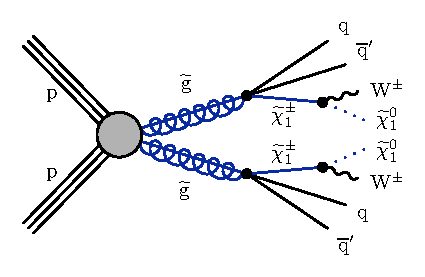
\includegraphics[width=0.5\textwidth]{Plots/feyndiagrams/T5qqqqWW.pdf}
\centering
  \caption{\label{fig:T5qqqqWW} Diagram showing the simplified model T5qqqqWW. 
  }
\end{figure*}

In the event selection, one of the $W$'s is chosen to be decaying leptonically. The choice of single lepton final states provides a cleaner event topology than the full hadronic final states while keeping the signal efficiency sufficiently high. Therefore, the visible final state includes at least six jets and one lepton (can be either electron or muon). Moreover, it is required that none of the jets are tagged as b quark to increase the probablity of selecting the events with topology T5qqqqWW. Furthermore, in such events, there is a momentum in balance originated by the neutralino and the neutrino which leave no trace in the detector. Therefore, a high missing transferse energy (MET) is also required. These selections can be further enhanced with the characteristics of individual objects such as; the transverse momentum of lepton $p_{T,\ell}$ or jets $p_{T, jets}$. 
However, only selecting events with one lepton, many jets, and high MET or using object characteristics is not enough to reveal the existence of SUSY-like events which are rare among the many SM like events with the similar final state. The $\wJets$ and $\ttJets$ events are the leading SM processes which can mimic the T5qqqqWW signature. Hence, some advanced kinematic variables need to be invented to eliminate these SM background processes. The table \ref{tab:KinVar} shows the list of variables which are used in this analysis. This list does not include the variables that are used in the identification of particle flow objects (see Sec. \ref{sec:PF}). The physics variables are categorised according to their mathematical complexity.\\
\renewcommand{\arraystretch}{1.5}
\begin{table}[ht]
\begin{center}
\begin{tabular}{|c|c|}\hline
Simple variables        & Advanced variables \\
\hline
\hline
$L_T$ , $H_T$ & $\Delta\Phi(W,\ell)$ \\
$p_{T,\ell}$ , $\eta_{\ell}$& $\MTt(\vec{p}_{\text T}^{\,\ell},\vec{p}_{\text T}^{\,t},\ptvecmiss)$  \\
$p_{T,jets\,(1,2)}$ & \\
$n_{jets}$ & \\
$n_{b-tag}$ & \\
\hline
\end{tabular}
\end{center}
\caption{List of kinematic variables}\label{tab:KinVar}
\end{table}
\renewcommand{\arraystretch}{1}
\subsection{Key variables}
\label{keyVars}
The list of simple variables consists of fundamental properties of the reconstructed physics objects, such as the transverse momentum $p_T$ of these objects, and their linear combinations.\\
%\boldmath
{\boldmath $L_{T}$} is the scalar sum of the charged lepton $p_T$ and the missing transverse momentum $E_T^{miss}$.
Given no additional source of $E_T^{miss}$, except the SM neutrino, the variable $L_T$ can be also written as: $\sqrt{p_{T(W)}^2+M_{T(W)}^2}$. The derivation of this relation is as follows:
\begin{eqnarray}
{p_{T(W)}^2} = {(p_{T(\ell)}\cdot cos\phi_{\ell} + \MET \cdot cos \phi_{\MET})^2+(p_{T(\ell)}\cdot sin\phi_{\ell} + \MET \cdot sin \phi_{\MET})^2},\nonumber \\
{M_{T(W)}^2} = {2\cdot p_{T(\ell)}\cdot\MET(1-(cos\phi_{\MET} \cdot cos\phi_{\ell} +sin\phi_{\MET}  \cdot sin\phi_{\ell} ))},\nonumber \\
{p_{T(W)}^2+M_{T(W)}^2}  = {p_{T(\ell)}^2+\MET^2+2\cdot p_{T(\ell)}\cdot\MET(cos\phi_{\MET} \cdot cos\phi_{\ell} +sin\phi_{\MET}  \cdot sin\phi_{\ell} )+2\cdot p_{T(\ell)}\cdot\MET},\nonumber \\
{(p_{T(\ell)}+\MET)^2} = {\LT^2}.
  \label{eq:LTderive}
\end{eqnarray}
For events with a single highly boosted $W$ boson ($p_{T(W)}\gg M_{T(W)}$), $L_T \sim p_{T(W)}$. This variable is also known as ``leptonic mass scale'' of the event. \\
{\boldmath $H_{T}$}  is the scalar sum of the transverse momenta of all jets above a $p_T$ threshold in the event. The major contribution to this sum is coming from transverse energy of the jets originated from the gluino decay, and it is related to the mass gap between the gluino and the chargino. This variable is reflecting the ``hadronic mass scale'' of the event. \\
{\boldmath $n_{jets}$} is the number of all jets  above a $p_T$ threshold, same as in the $H_T$ calculation, in the event.\\
{\boldmath $n_{b-tag}$} is the number of all jets tagged as coming from a b quark above a $p_T$ threshold, same as with other jets, in the event.\\
The other variables in the list such as $p_T,\ell$ or $\eta_{\ell}$ was discussed in Sec. \ref{sec:PF} regarding particle flow objects.\\
There are two advanced variables used in this analysis.\\
{\boldmath $\Delta\Phi(W,\ell)$} is the azimuthal angle between the $W$ boson and the charged lepton. In the $\wJets$ and $\ttJets$ events, the lepton comes from a leptonic decay of $W$ boson, $W\rightarrow\ell\nu$. Therefore, $\Delta\Phi(W,\ell)$ strongly related to the mass of the $W$ boson and its momentum. In SM events with high missing energy indicates that the $W$ bosons yielding the lepton and the neutrino are boosted, hence resulting in a narrow distribution in $\Delta\Phi(W,\ell)$. On the other side, in SUSY decays, the missing transverse energy comes from two neutralinos and the neutrino, which randomizes the  $\Delta\Phi(W,\ell)$, thus resulting in an even distribution in $\Delta\Phi(W,\ell)$. As a result of its features, the variable $\Delta\Phi(W,\ell)$, is the most significant variable in this analysis. The high values of $\Delta\Phi(W,\ell)$ is used as a signal region\footnote{where signal to background event counts are sufficiently large.} while the low values of $\Delta\Phi(W,\ell)$ is the control region\footnote{where signal event counts are negligible with respect to background event counts.}.\\
{\boldmath $\MTt$}  is defined as:
\begin{eqnarray}
  \MTt(\vec{p}_{\text T}^{\,\ell},\vec{p}_{\text T}^{\,t},\ptvecmiss) =
  \min\limits_{\vec{p}_{\text T}^{(1)}+\vec{p}_{\text T}^{(2)} = \ptvecmiss} \left\{
  \max \left[ \MT(\vec{p}_{\text T}^{\,\ell}, \vec{p}_{\text T}^{(1)}), 
              \MT(\vec{p}_{\text T}^{\,t},\vec{p}_{\text T}^{(2)})\right] \right\},
  \label{eq:MT2}
\end{eqnarray}
where $\MT$ is the transverse mass and the indices $t$,$\ell$ represent isolated track and the selected lepton repectively. In this analysis, this variable is used only in the baseline selection to reduce the dileptonic $\ttJets$ contribution which is more important in the signal region (high  $\Delta\Phi(W,\ell)$). 
\subsection{Signal samples}
\label{signalSamples}
The simplified model T5qqqqWW is discussed in section  \ref{sec:simplifiedModels}. This model originally includes three free parameters: the masses of the gluino $m_{\tilde{g}}$, the intermediate chargino $m_{\chipmone}$ and the neutralino $m_{\ninoone}$. To reduce the three dimension mass space the chargino mass is fixed to midway between gluino and neutralino mass. Hence, this model is investigated in the $m_{\tilde{g}}$-$m_{\ninoone}$ mass plane. For each mass point, a separate Monte Carlo sample is produced. The mass plane is shown in  Fig. \ref{fig:massplane} where the z-axis represents the total number of events generated. This scan of parameter space includes 657 mass points and it requires more computational power than usual SM process production therefore fastsim is used as explained in section \ref{fastsim}. The MADGRAPHv5 event generator is used for signal events modelling. The samples are normalized to the cross section presented by the LHC SUSY Cross Section Working Group \cite{gluxsec2}.
Throughout present thesis, two mass points corresponding to different gluino and neutralino masses are used as benchmarks to study the kinematic properties of the signal. 
\\
\textbf{T5qqqqWW(1.9,0.1)} represents a point in the high mass gap region with $m_{\tilde{g}}=$ 1900 GeV and $m_{\ninoone}=$ 100 GeV. These signal events have high \HT and \LT.
\\
\textbf{T5qqqqWW(1.5,1.0)} represents a point close to the compressed region with $m_{\tilde{g}}=$ 1500 GeV and $m_{\ninoone}=$ 1000 GeV.  The compressed region is where the $m_{\tilde{g}}-m_{\ninoone}\leq2m_{W}$. These signal events have lower \HT and \LT with respect to high mass gap ones.

\begin{figure*}[!hb]
  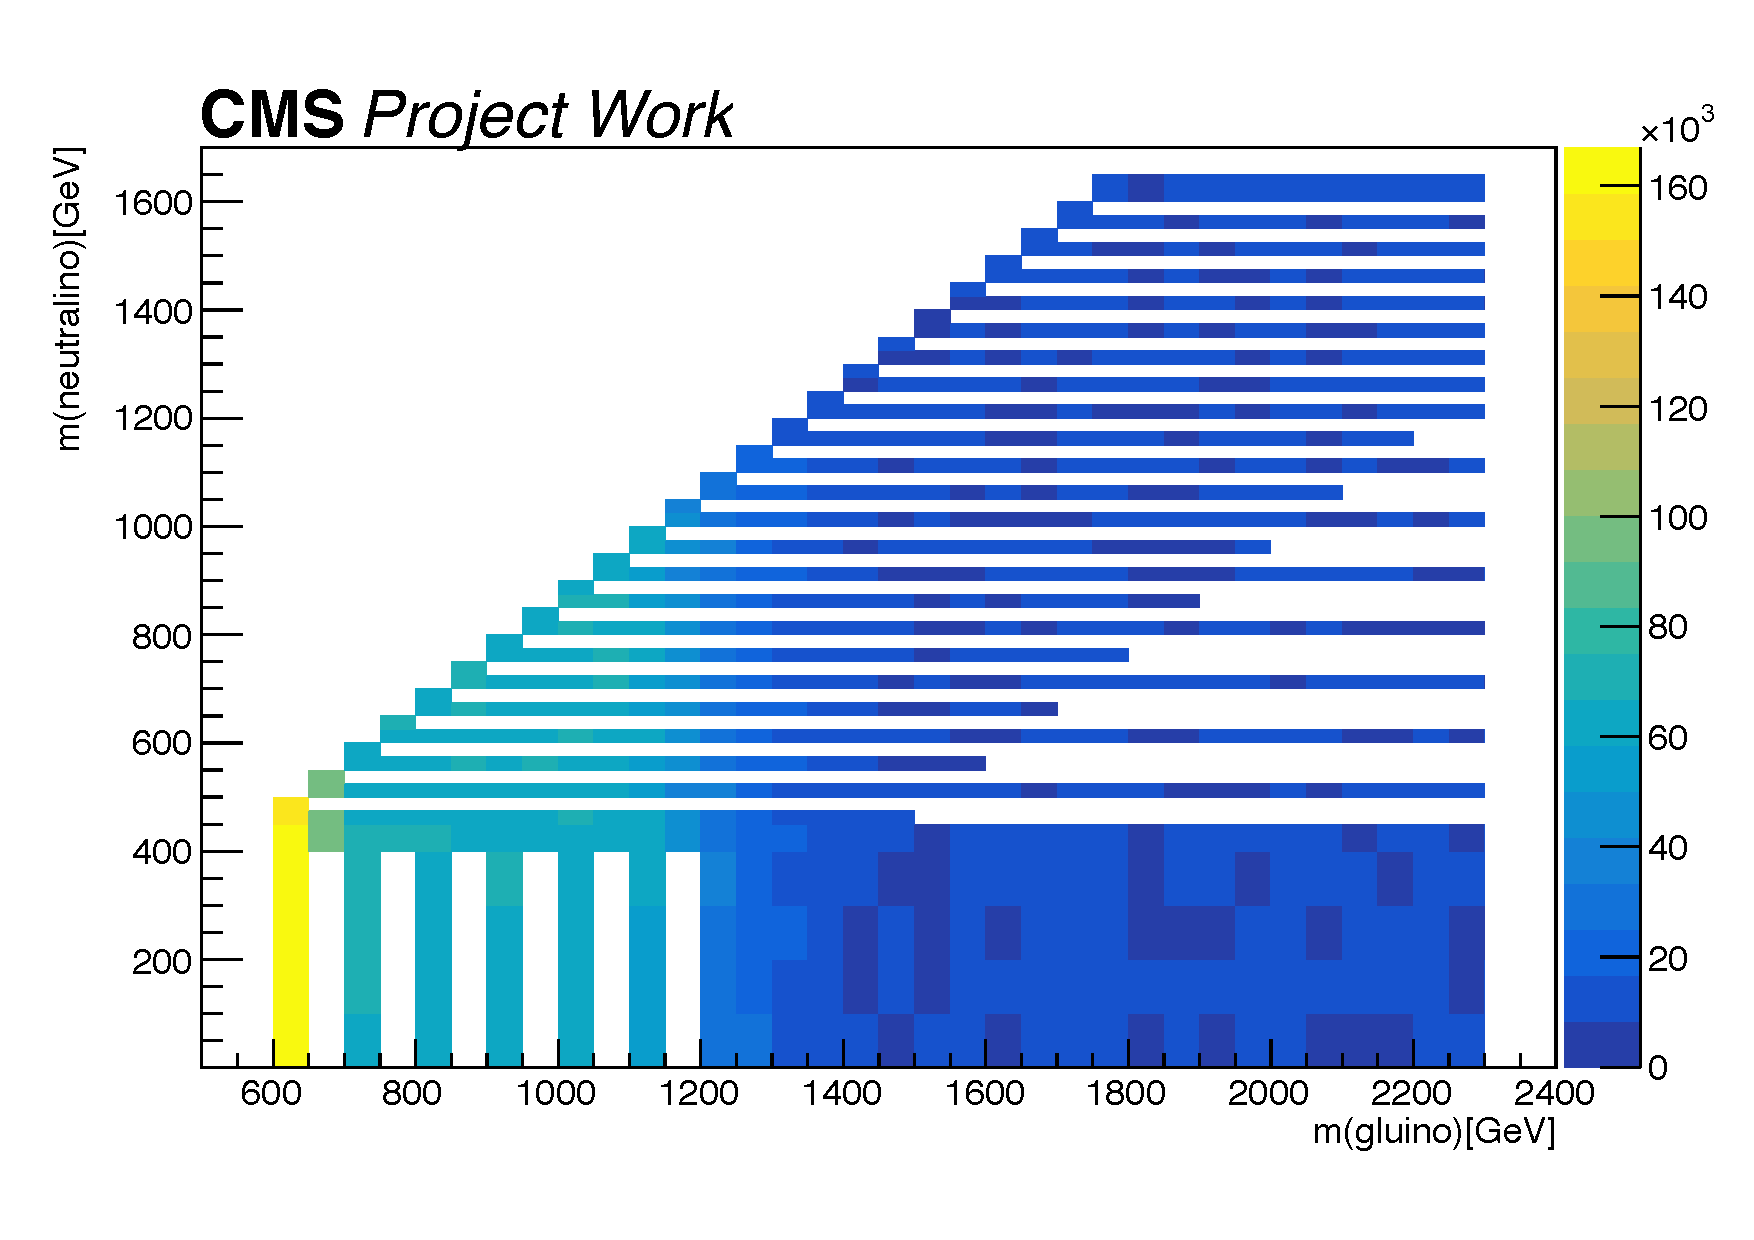
\includegraphics[width=0.7\textwidth]{Plots/signals/signal_scan.pdf}
\centering
  \caption{\label{fig:massplane} Produced signal mass points for the simplified T5qqqqWW model. 
  }
\end{figure*}

%\section{Samples}
\section{Background processes}
\label{sec:bkg_proc}
As mentioned earlier in this section the most important background processes are $\wJets$ and $\ttJets$ events. Requiring zero b-tagged jets in the event selection, $\wJets$ events becomes the main background. All of the background processes considered in this analysis are listed below. PYTHIA 8 is used for parton shower and hadronisation. \\
%\begin{aligned}
{\boldmath $\ttJets$} is generated with $\MADGRAPH$5\_\textsc{aMC@}NLOv2.2.2. To enhance the statistics the combination of $\HT$ binned samples, dedicated semi- and dilep- tonic samples is used.\\
{\boldmath $\wJets$} is generated with $\MADGRAPH$5\_\textsc{aMC@}NLOv2.2.2. $\HT$ binned samples, where $W$ decaying leptonically, are used.\\
\textbf{QCD multijets} events are produced with $\MADGRAPH$5\_\textsc{aMC@}NLOv2.2.2 in bins of $\HT$.\\
{\boldmath $\singleTop$} samples are produced with POWHEGv2.0 except the $t$ decaying leptonically with s-channel is produced with NLO $\MADGRAPH$5\_\textsc{aMC@}NLOv2.2.2. \\
\textbf{\DY} evemts are produced with $\MADGRAPH$5\_\textsc{aMC@}NLOv2.2.2 and $m_{\ell\ell}>50 GeV$ samples are used in $\HT$ bins.\\
\textbf{Di-boson} samples are produced with AMC$@$NLO except $WW$ samples are produced with powheg.\\
{\boldmath \TTVH} samples are produced with  AMC$@$NLO.\\
A list of all background MC samples with cross sections can be found in Appendix \ref{sec:Appsamples}.
%\end{aligned}
%\newpage
\subsection{Scale Factors}
\label{sec:SF}
The modeling of physics processes and the simulation of the detector responses are not perfect. Studies of the data-MC discrepancies indicate that MC needs to be corrected by some event-by-event weights, which are called scale factors. The scale factors used in this analysis are as follows:\\
\textbf{Lepton identification and reconstruction efficiency:}\\
MC samples have to be corrected according to the reconstruction and identification efficiencies of leptons.
In this work, scale factors are applied as a function of $p_{T}$ and $\eta$ of the selected lepton. They are calculated for electrons and muons separately by the e-gamma and muon physics object groups respectively\cite{leptonSF}.\\
\textbf{B-tagging efficiency:}\\
The simulated b-tagging efficiency is corrected with respect to the one in data. For each simulated event, weights corresponding to the different number of b-tagged jets values are calculated and this results in multiple weights for each event\cite{leptonSF}. This method allows reusing the events. The advantage of this method is that it provides to use full statistical power of the MC events.\\
\textbf{ISR reweighting:}\\
Since the 8 TeV Run of LHC, it is known that the $p_T$ spectrum of $\ttbar$ events are not well modeled. Therefore, an event-by-event correction is obtained using the jets from initial state radiation (ISR).
 In the present analysis, each event is corrected according to number of ISR jets. The weights can be seen in table \ref{tab:nISRweights} where the D factor is for keeping the normalization of the overall sample invariant. This D factor is calculated using an inclusive sample i.e. without the specific selections of the analysis.
 \renewcommand{\arraystretch}{1.5}
\begin{table}[htbp]
\begin{center}
\caption{Weights based on the number of ISR jets as given in Ref.~\cite{nISRweightTTbar}}
\begin{tabular}{|r|l|}
\hline
\multicolumn{1}{|l|}{nISR jet} & Normalisation weight $D_{\ttbar} = 1.071$ \\ \hline
0 &  \\ \hline
1 & $D \times (0.920 \pm 0.005 \pm 0.040)$ \\ \hline
2 & $D \times (0.821 \pm 0.006 \pm 0.090)$ \\ \hline
3 & $D \times (0.715 \pm 0.009 \pm 0.143)$ \\ \hline
4 & $D \times (0.662 \pm 0.016 \pm 0.169)$ \\ \hline
5 & $D \times (0.561 \pm 0.027 \pm 0.219)$ \\ \hline
$\geq$ 6& $D \times (0.511 \pm 0.041 \pm 0.244)$ \\ \hline
\end{tabular}
\label{tab:nISRweights}
\end{center}
\end{table}
\\
\renewcommand{\arraystretch}{1}
\textbf{Pileup:}\\
As discussed earlier in Section \ref{sec:PrimaryVert}, the number of pile-up interactions in simulated samples is generated with a prior distribution. Thus, the MC pile-up distribution may vary from the actual pile-up distribution in Data. The simulated distribution is rescaled with the Data/MC ratio in Figure \ref{fig:pileUpmine}.
\begin{figure*}[!hb]
  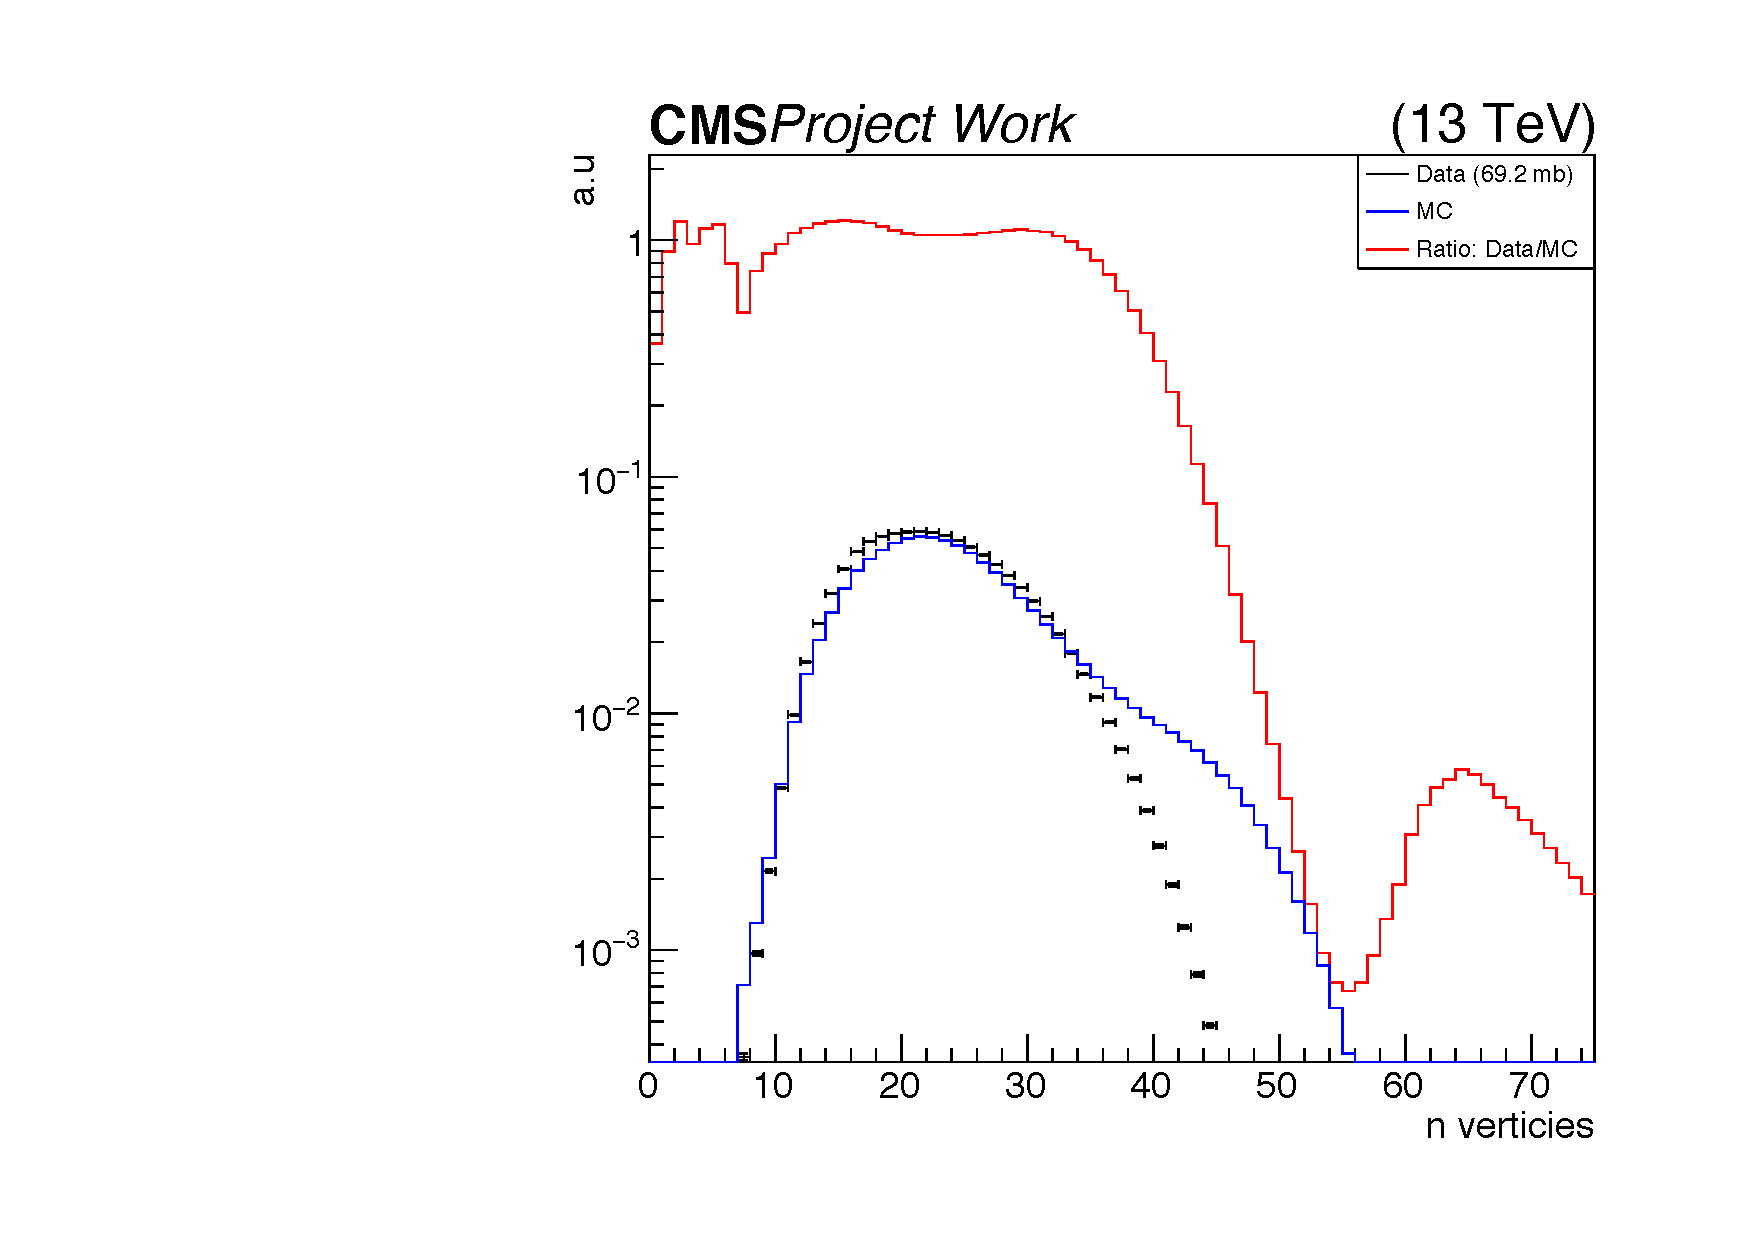
\includegraphics[width=0.6\textwidth]{Plots/analysis/pileUp/pileUp.pdf}
\centering
  \caption{\label{fig:pileUpmine} The normalised distributions of mean number of interactions per bunch crossing during the analysed data Run2016 (black) and in the MC samples (blue). And the red distribution represents the Data to MC ratio. For the data distribution the latest luminosity calibrations ~\cite{PileUp} and an inelastic pp cross-section of 69.2 mb are used. 
  }
\end{figure*}\\
\section{Baseline selection}
\label{sec:BL}
Earlier in this section \ref{signalDef}, the SUSY signature considered in this work is introduced. Moreover, a suitable primary event selection for removing the SM background as much as possible while keeping the signal efficiency high was discussed. In the following, details of this event selection are explained.\\
\textbf{Selection of leptons:}\\
The selected lepton, which can be an electron or a muon, is required to have a minimum $\pt$ of 25 GeV while at the same time it satisfies the good lepton criteria introduced in Sec. \ref{sec:PF}. Additionally, all the other electrons and muons with $\pt$ greater than 10 GeV are vetoed. These veto leptons satisfy the loose lepton selection with $I_{rel}<0.4$.
\\
\textbf{Selection of jets:}\\
The reconstruction of jets is already introduced in Sec. \ref{sec:PF}. In the present analysis, jets are required to have $\pt > 30$ GeV and $| \eta | < 2.4 $. In order to avoid double counting of objects, jets that are close ($\Delta R <0.4$) to either a veto or selected lepton are removed.
As discussed earlier in this chapter the T5qqqqWW is expected to have at least five jets. Moreover, the mass difference of the gluino and the intermediate chargino affects the $\pt$ of the jets. Therefore, it is required that two highest $\pt$ jets satisfy the $\pt >80$ GeV condition. Additionally, in the baseline selection of the analysis, the number of jets tagged as coming from b quarks is zero to suppress the events containing top quarks.
\\
\textbf{Energy scales thresholds:}\\
The signal model considered in this work favors events with high hadronic and leptonic scale. The hadronic scale is chosen to be at least 500 GeV while the leptonic scale threshold is 250 GeV.
\\
\textbf{Isolated track veto:}\\
The isolated track veto is designed to suppress $\ttbar$ events in which both W bosons decay leptonically and one lepton does not satisfy the selection criteria for veto leptons. In the mechanism of this veto, the $\MTt$ variable, which is introduced in section \ref{keyVars}, is used with an isolated track $\vec{t}$, a lepton $\vec{\ell}$ and the missing transverse momentum $\ptvecmiss$. In the calculation of $\MTt$, it is assumed that the missing energy source is the two neutrinos from the dileptonic $\ttbar$ decay. The minimization runs over all possible splitting of $\ptvecmiss$.
The figure \ref{fig:track_mt2} shows the $\MTt$ distribution seperate for hadronic and leptonic tracks after the baseline selection with $\HT > 500$ GeV, $\LT > 250$ GeV,  $\njet \geq 5$ and without b-tag requirement. The distribution of
\MTt\, is slightly different for the two cases and a lower \MTt\, cut of $60$ GeV and $80$ GeV is
applied for hadronic and leptonic tracks respectively. The rightmost plot in  the figure ~\ref{fig:track_mt2}
shows the \MTt\, distribution for all events i.e. including events that do not have any isolated track at
all. In this case events without any isolated track are added to the overflow bin. It can also be derived from the plot that only about 20\% of the signal events have an opposite charged isolated track at all compared to 40\% of the dileptonic $\ttbar$ events.
 \begin{figure*}[!hbt]
    \begin{center}
  \subfigure[\MTt\, with leptonic tracks]{ 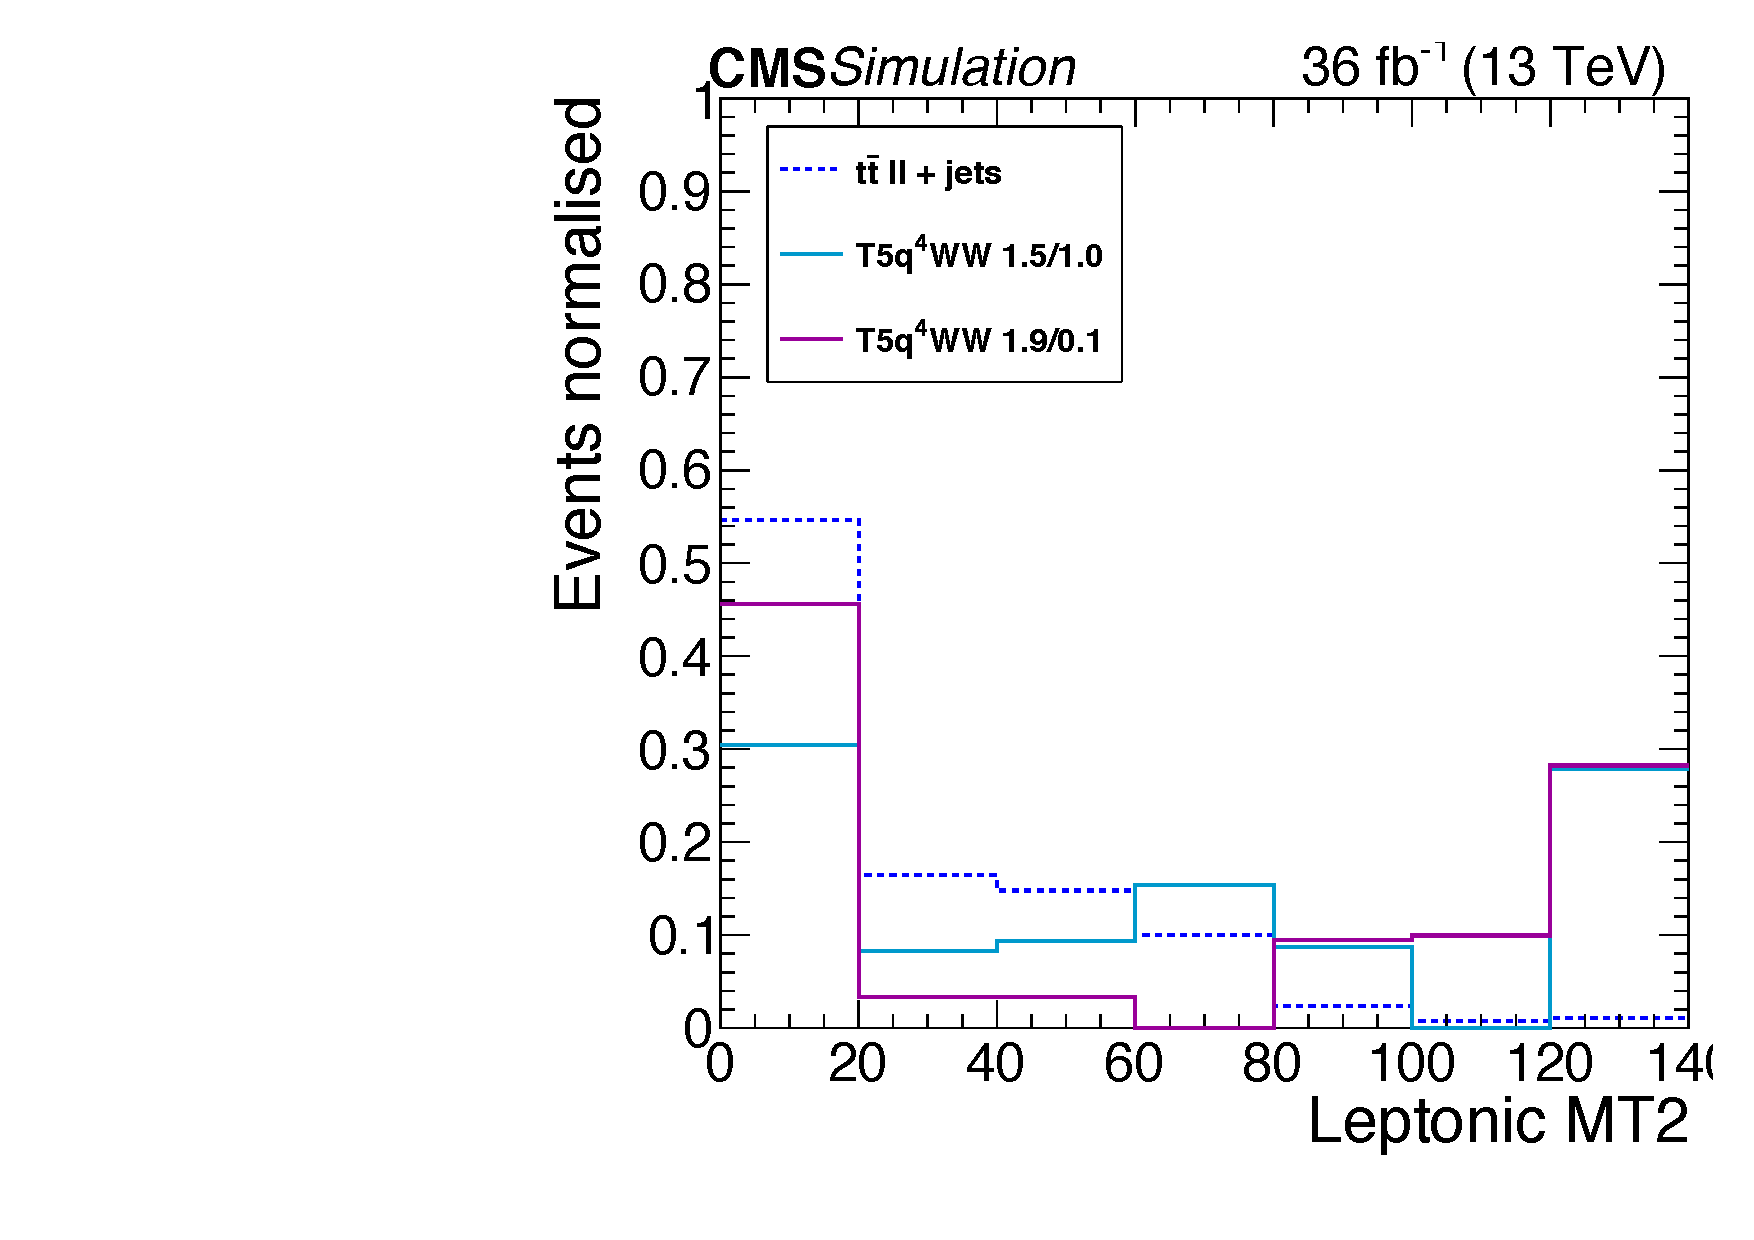
\includegraphics[width=0.3
    \textwidth]{Plots/analysis/isoveto/Mt2_nobReq_LEP.pdf}}
    \subfigure[\MTt\, with hadronic tracks]{ 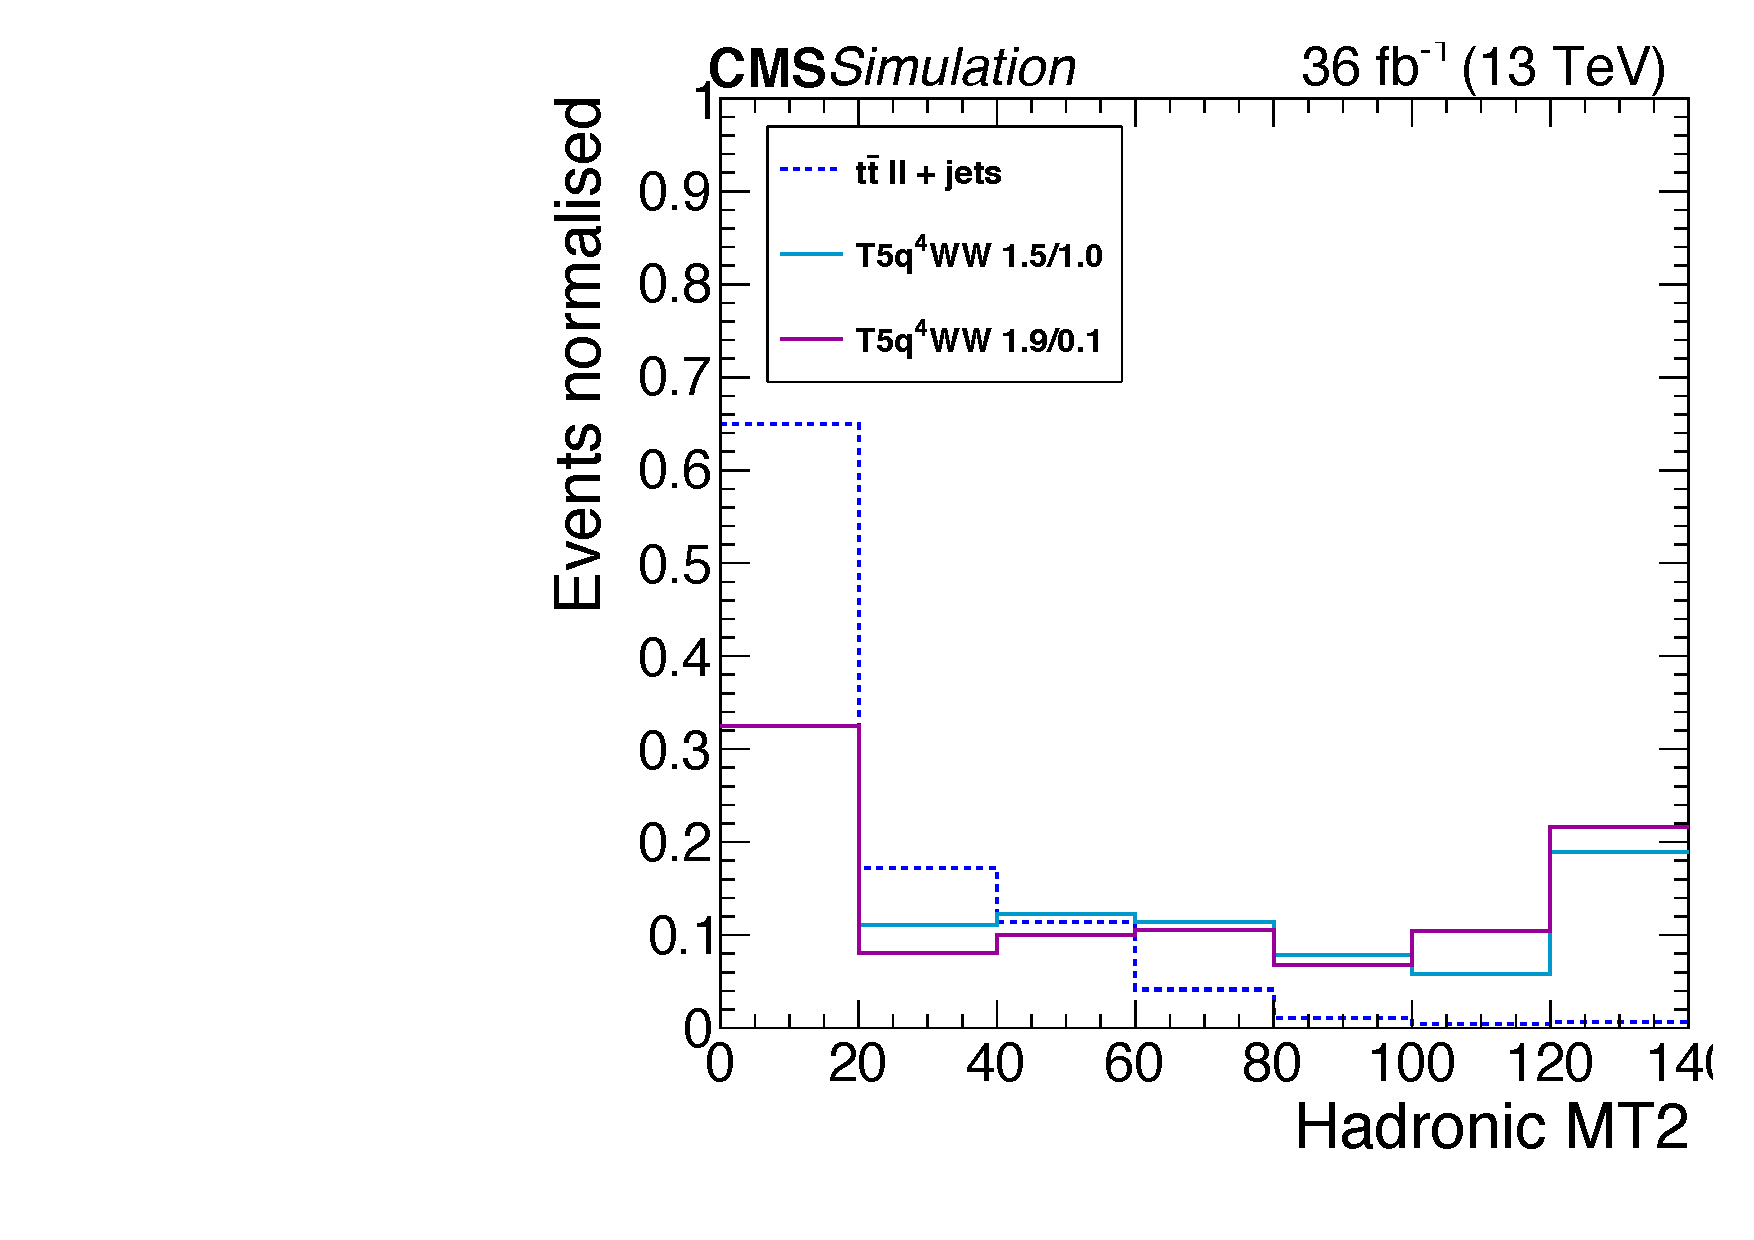
\includegraphics[width=0.3
    \textwidth]{Plots/analysis/isoveto/Mt2_nobReq_HAD.pdf}}
    \subfigure[\MTt\, (All events)        ]{ 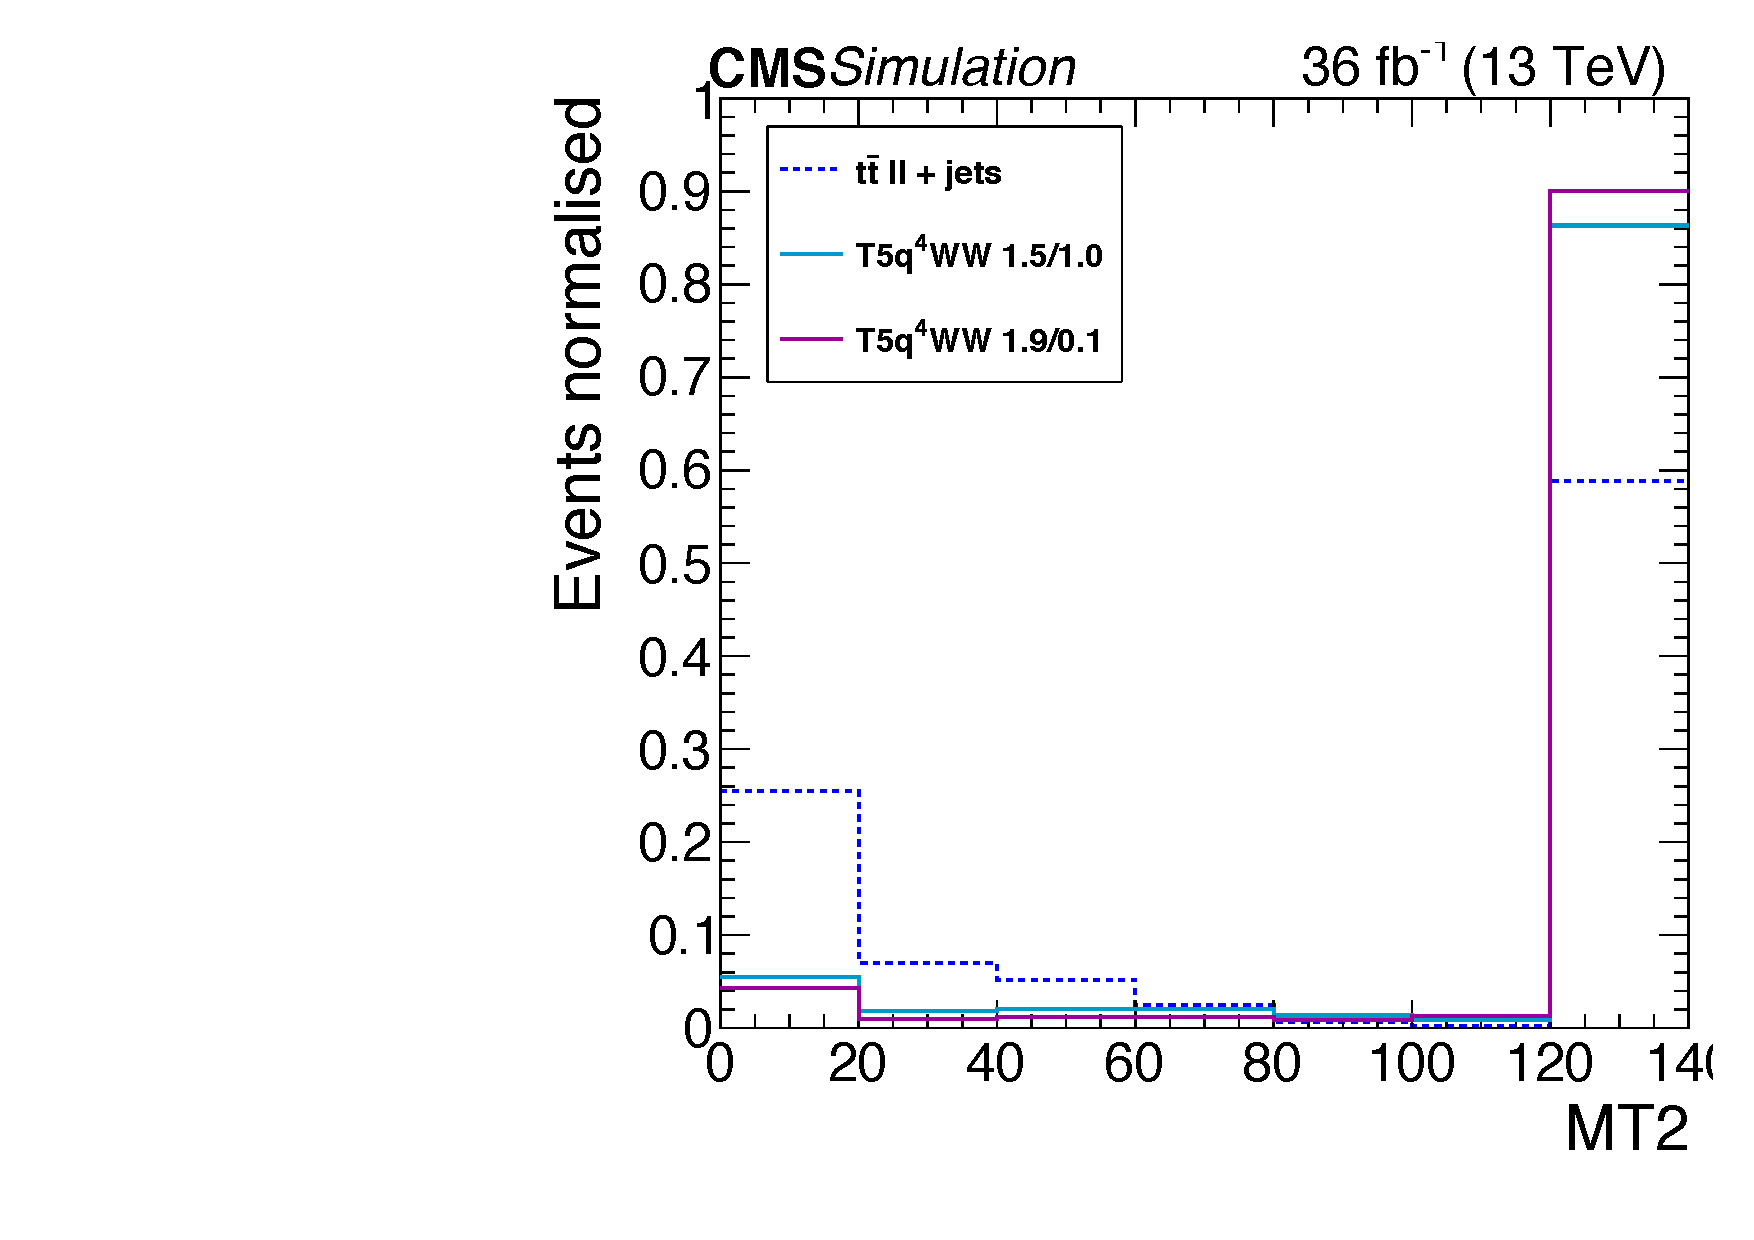
\includegraphics[width=0.3
    \textwidth]{Plots/analysis/isoveto/Mt2_nobReq_ALL.pdf}}
  \caption{ \label{fig:track_mt2} Distributions of $\MTt$ for events with electron or muon veto tracks (a) and hadronic veto tracks (b), for dileptonic $\ttbar$ (blue dotted) and T5qqqqWW (purple and azure) signal samples. The highest bin is always an overflow bin. The majority $\ttbar$ events have $\MTt < 80$ GeV, while the signal events have longer
    tails in $\MTt$.
    The rightmost plot (c) shows the distribution for all events. 
  }
   \end{center}
\end{figure*}
\\
The effect of each baseline requirement is demonstrated in Figure \ref{fig:plotFlow} for the different background processes (stacked) and for two signal benchmark points. It should be noted that the background samples include an initial skim of $\HT > 350$ GeV and $\LT > 150$ GeV to shorten the computation time. It can be observed that the design of baseline selections works such that they reduced the background events significantly while only a small fraction of signal events are eliminated by the selections. It can be also notted that, naturally, the QCD background is almost vanished after the single muon selection. The estimation of important backgrounds will be explained in the next chapter.
\renewcommand{\arraystretch}{1.5}
\begin{table}[ht]
\begin{center}
\begin{tabular}{|c|c|}\hline
Selection        & Object definitions \\
\hline
\hline
Single lepton &Tight leptons, $\pt \geq 25$ GeV and $|\eta| < 2.4$\\
                      & and $I_{mini}<0.1(0.2)$ for electrons(muons)\\\hline
Lepton veto & Loose leptons, $\pt \geq 10$ GeV and $|\eta| < 2.4$ \\
		& and $I_{mini}<0.4$ \\\hline
Isolated track veto & $I_{rel}<0.3$, $\Delta R(\ell,track) <0.1$, charge$_{track}$ = -charge$_{lepton}$  \\\hline
$n_{jets} \geq 5$ & Good jets with $\pt \geq 30$ GeV and $|\eta| < 2.4$ \\
\cline{1-1}
$p_{T,jets\,(1,2)} \geq 80$ GeV & and cleaned from close leptons \\\hline
$H_T \geq 500$ GeV & $\sum_{jets} \pt$\\\hline
$L_T \geq 250$ GeV &  $\MET + \pt^{lep}$ \\\hline
$n_{b-tag} = 0$ & b-tagged good jets with CSVv2 Medium working point (0.8484)\\\hline
\end{tabular}
\end{center}
\caption{List of event selection criteria and object requirements.}\label{tab:CutSummary}
\end{table}
\renewcommand{\arraystretch}{1}
 \begin{figure*}[!hbt]
    \begin{center}
    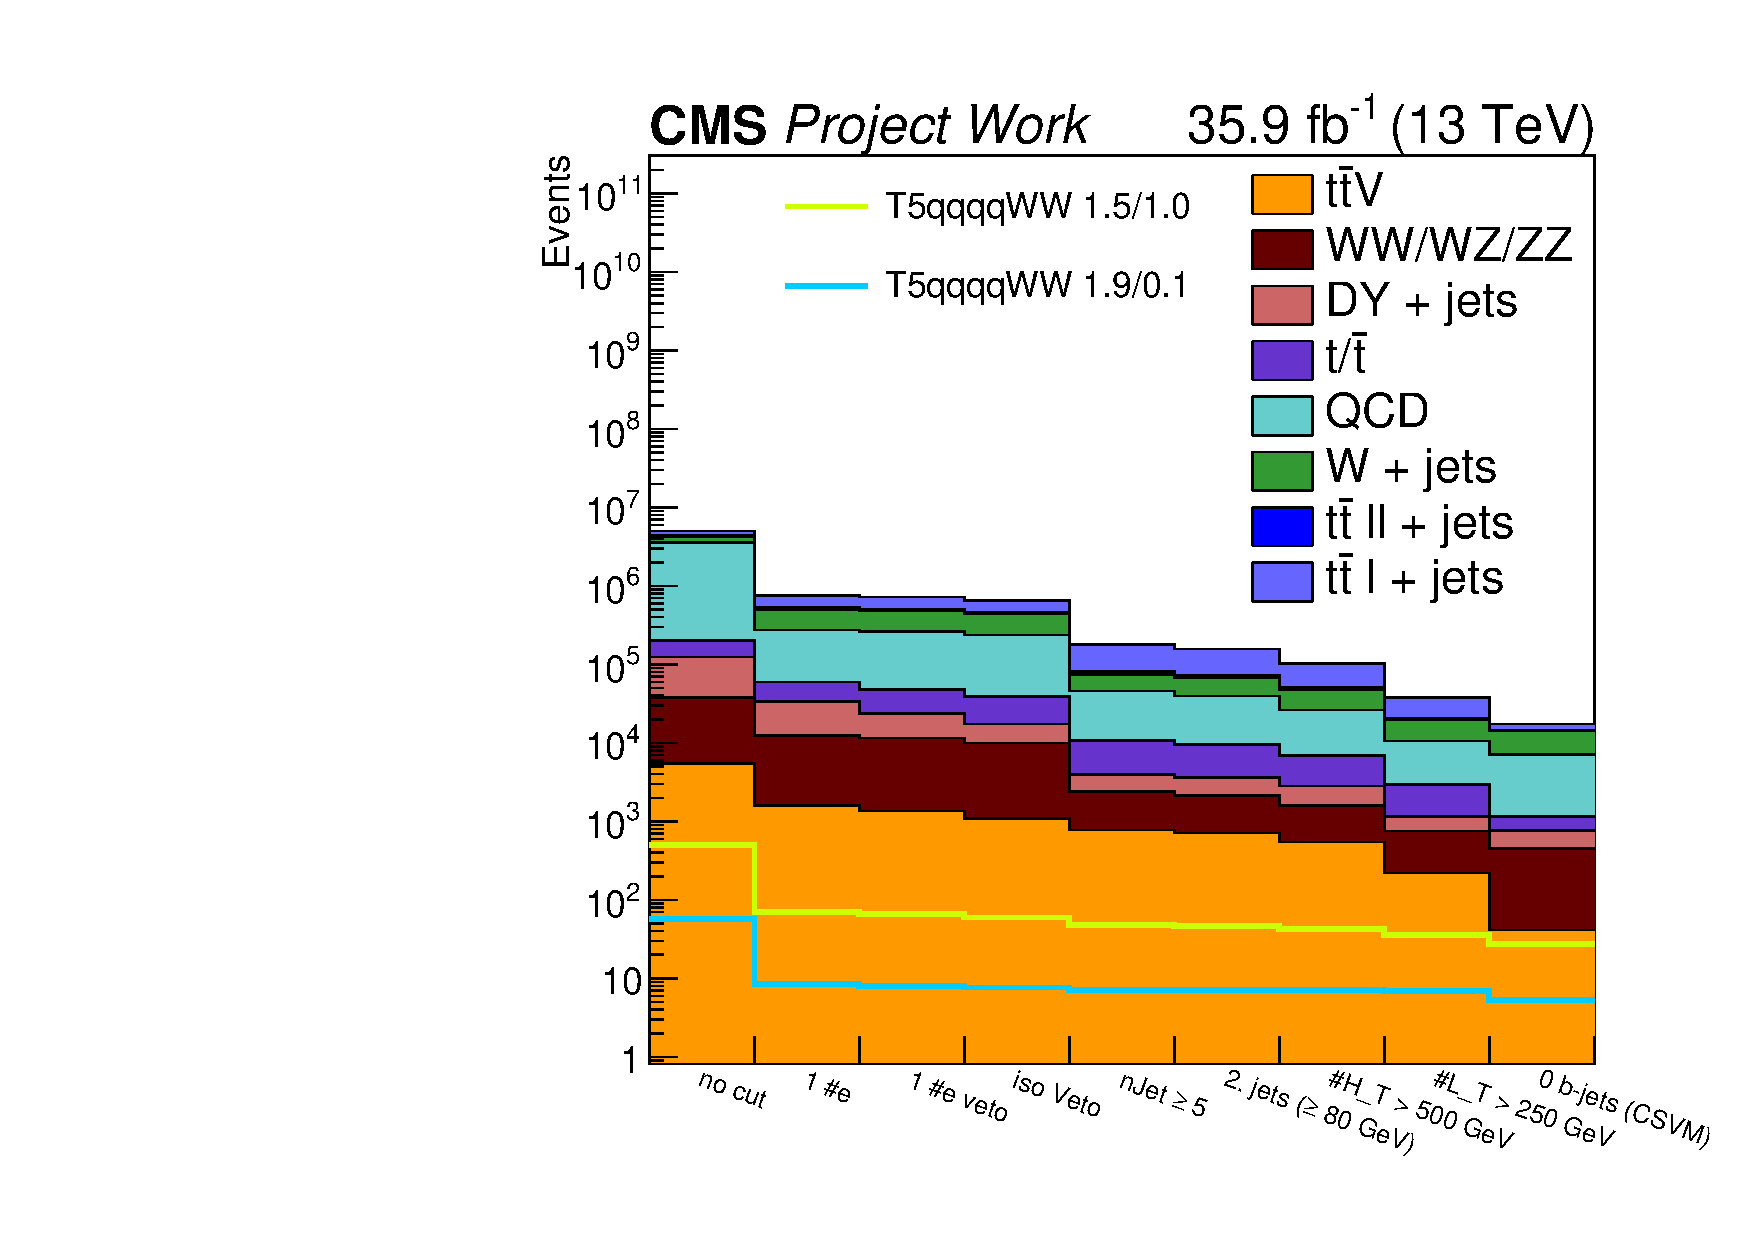
\includegraphics[width=0.45\textwidth]{Plots/analysis/cutflow/electron}
     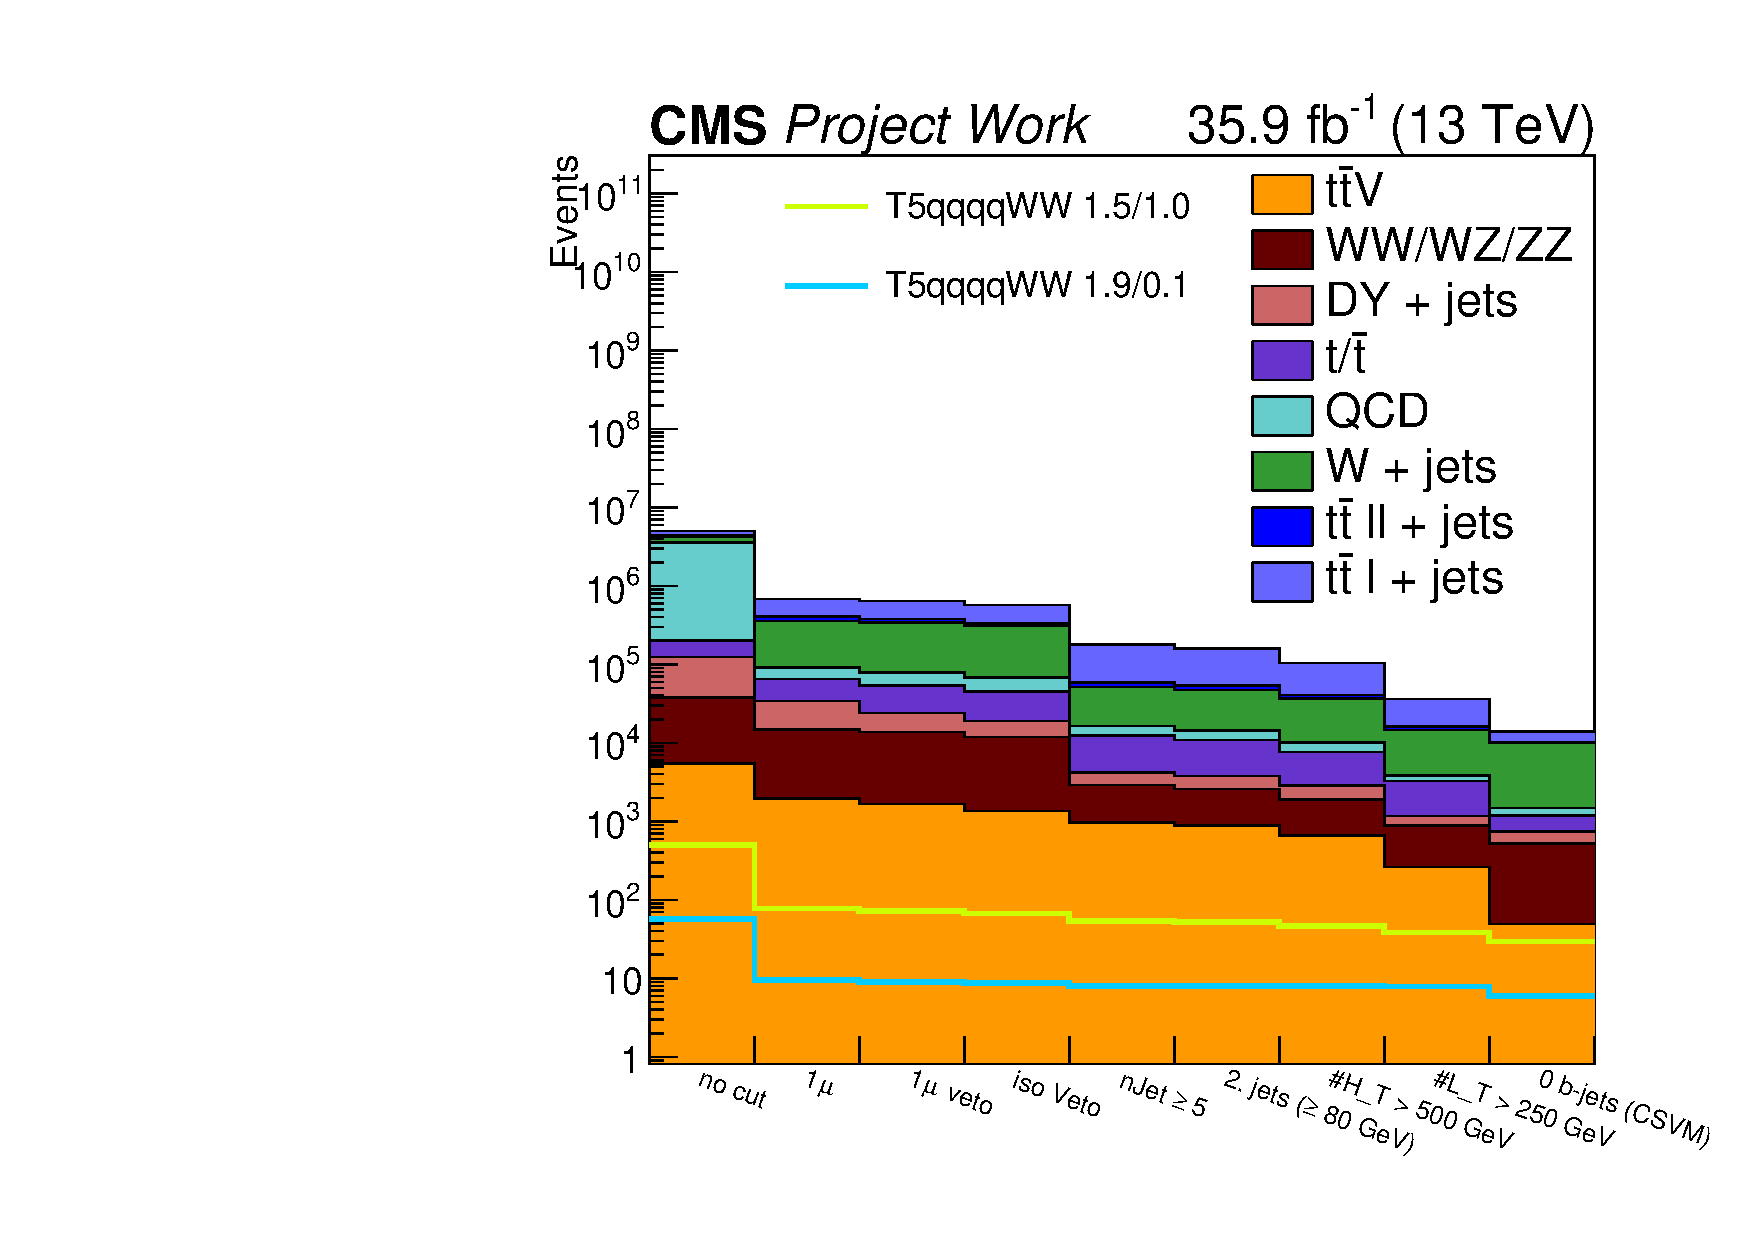
\includegraphics[width=0.45\textwidth]{Plots/analysis/cutflow/muon}
  \caption{ \label{fig:plotFlow} The number of events for each sample for the electron (left) and muon (right) channel. Samples are scaled to the luminosity with their cross section and scale factors discussed in section \ref{sec:SF}.
  }
   \end{center}
\end{figure*}
\section{Data Samples}
The data used for this analysis is recorded by the CMS detector during the 2016 LHC run at 13 TeV.  As in Figure \ref{CMSlumi},   The total integrated luminosity collected by CMS is 37.76 fb$^{-1}$. In the present analysis, the data validated by the CMS Data Quality Monitoring (CMS-DQM) certification team, which correspond to an integrated luminosity of L=35.9 fb$^{-1}$, is used. 
\subsection{Triggers}
\label{sec:triggers}
In this analysis, the main trigger set is a combination of triggers containing an isolated single lepton, electron or muon, with pT of 15 GeV and HT of 350/400 GeV.  To recover inefficiencies due to an update on the online electron ID and the saturated L1-jets, the trigger strategy had to be extended: The list of trigger paths can be seen in Table \ref{tab:triggers}.
\renewcommand{\arraystretch}{1.5}
\begin{table}[ht]
\begin{center}
\begin{tabular}{|c|}\hline
Single Electron Dataset \\
\hline
\hline
      HLT\_Ele105\_CaloIdVT\_GsfTrkIdT\_v \\
      HLT\_Ele115\_CaloIdVT\_GsfTrkIdT\_v \\
      HLT\_Ele50\_CaloIdVT\_GsfTrkIdT\_PFJet165\_v \\
      HLT\_Ele27\_WPTight\_Gsf\_v \\
      HLT\_Ele15\_IsoVVVL\_PFHT350\_v \\
      HLT\_Ele15\_IsoVVVL\_PFHT400\_v \\
\hline
Single Muon dataset \\
\hline
\hline
      HLT\_Mu50\_v \\
      HLT\_IsoMu24\_v \\
      HLT\_IsoTkMu24\_v \\
      HLT\_Mu15\_IsoVVVL\_PFHT350\_v \\
      HLT\_Mu15\_IsoVVVL\_PFHT400\_v \\
\hline
MET dataset \\
\hline
\hline
      HLT\_PFMET100\_PFMHT100\_IDTight\_ OR  HLT\_PFMETNoMu100\_PFMHTNoMu100\_IDTight\_ \\
      HLT\_PFMET110\_PFMHT110\_IDTight\_ OR  HLT\_PFMETNoMu110\_PFMHTNoMu110\_IDTight\_  \\
      HLT\_PFMET120\_PFMHT120\_IDTight\_ OR HLT\_PFMETNoMu120\_PFMHTNoMu120\_IDTight\_  \\
\hline
\end{tabular}
\end{center}
\caption{List of HLT paths}\label{tab:triggers}
\end{table}
\renewcommand{\arraystretch}{1}
Events recorded with these trigger paths are allocated in three primary datasets (PDs): the \textbf{SingleElectron}, \textbf{SingleMuon} and \textbf{MET} datasets.
Therefore, when successively adding PDs, triggers contained in previous PDs are vetoed to avoid double counting of events contained in more than one of the PDs.
The trigger efficiency calculation is shown in the Equation \ref{Eqtrig}. The trigger efficiencies are measured as a function of \LT, \, \HT\, and lepton $p_T$ and can be seen in Figures \ref{fig:trig_eff_LT}, \ref{fig:trig_eff_HT}, \ref{fig:trig_eff_leptonPt} respectively.
The efficiency distribution in the baseline region (\LT$>$250 GeV; \HT$>$500 GeV; lepton $p_T$ $>$25 GeV) is flat and its value close to 100\%(98\%) for the muons (electrons).
\begin{equation}
\label{Eqtrig}
  \epsilon = \frac{N({\rm all \; events \; passing \; probed \; trigger(s) +
  preselection + reference \; trigger})}{N({\rm all \; events \; passing
  \;preselection + reference \; trigger})}
\end{equation}

\begin{figure*}[!hbt]
  \begin{center}
    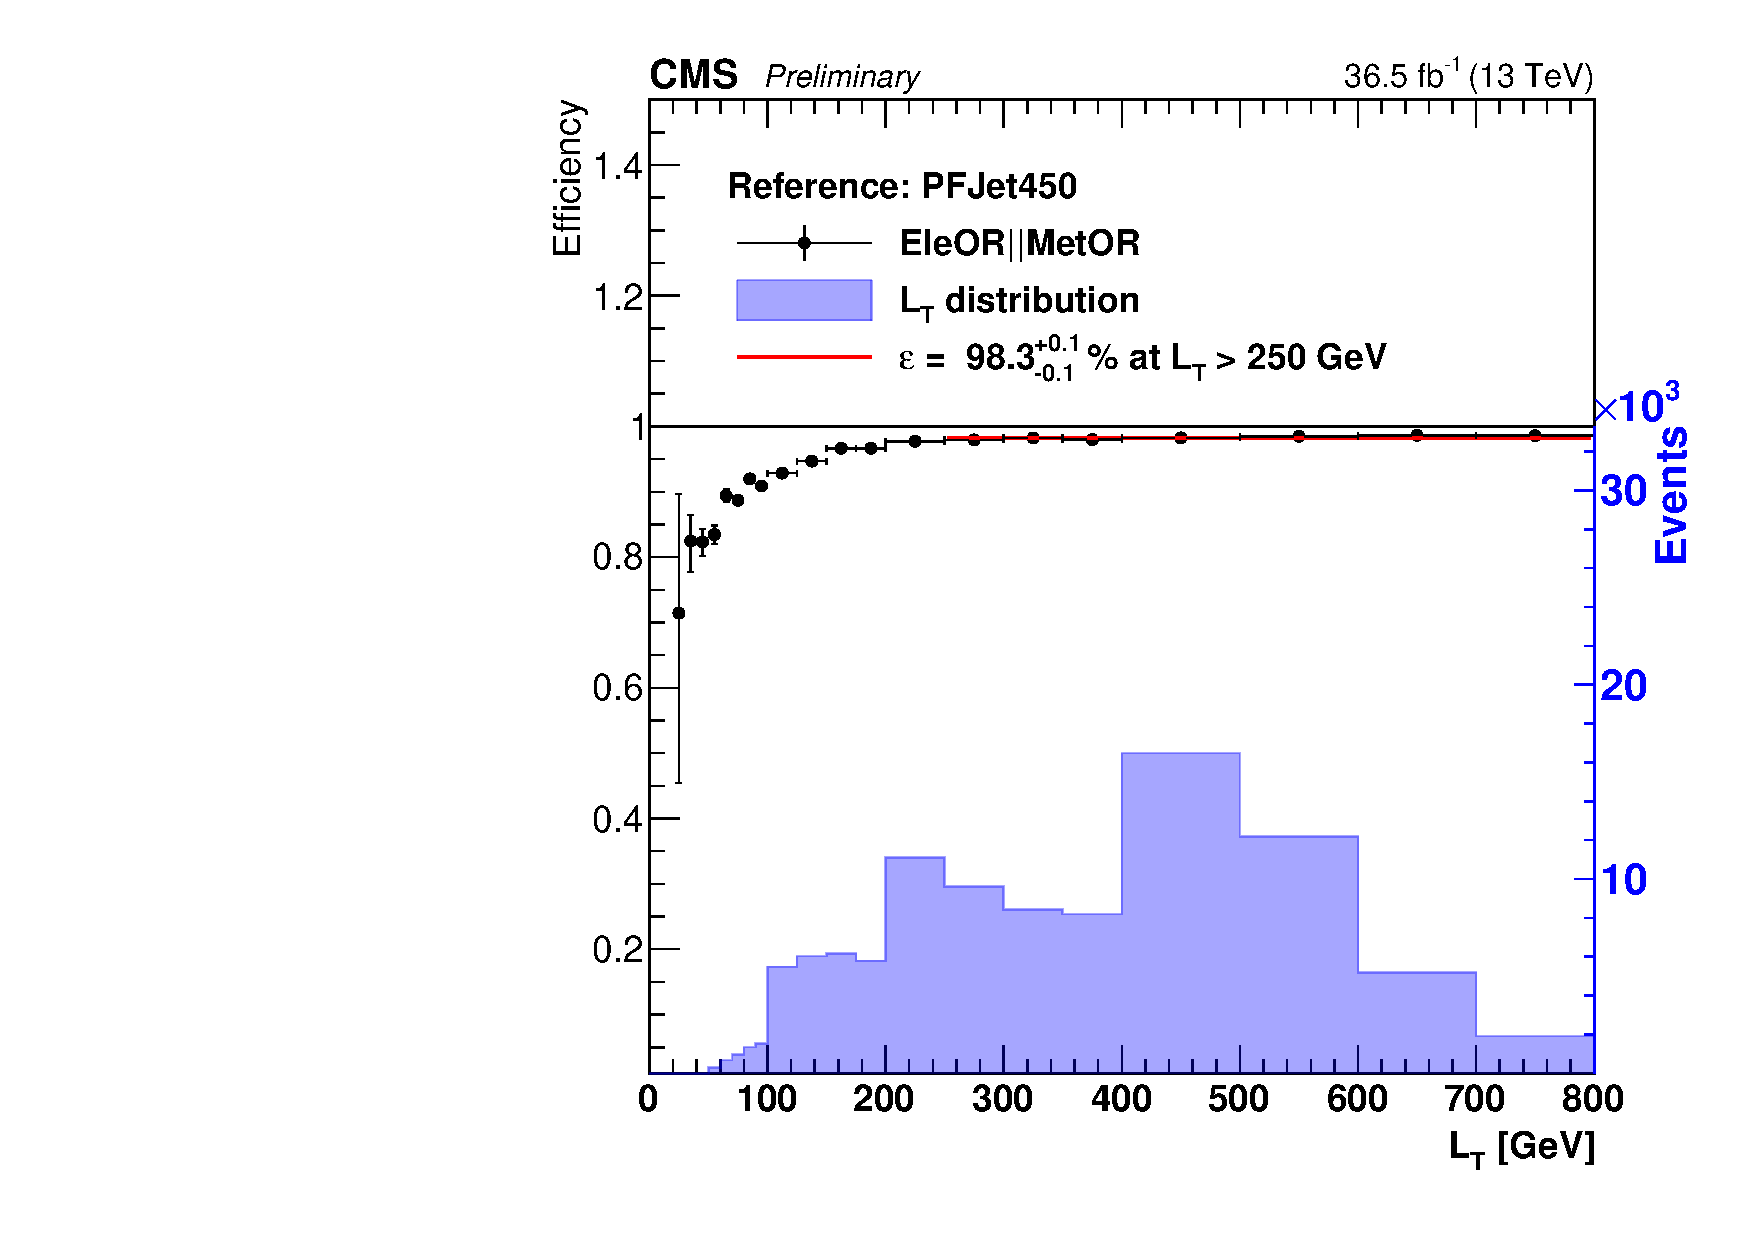
\includegraphics[width=0.4\textwidth]{Plots/trigger/LT_PFJet450_EffFit_test_HLT_EleORORHLT_MetOR.pdf}
    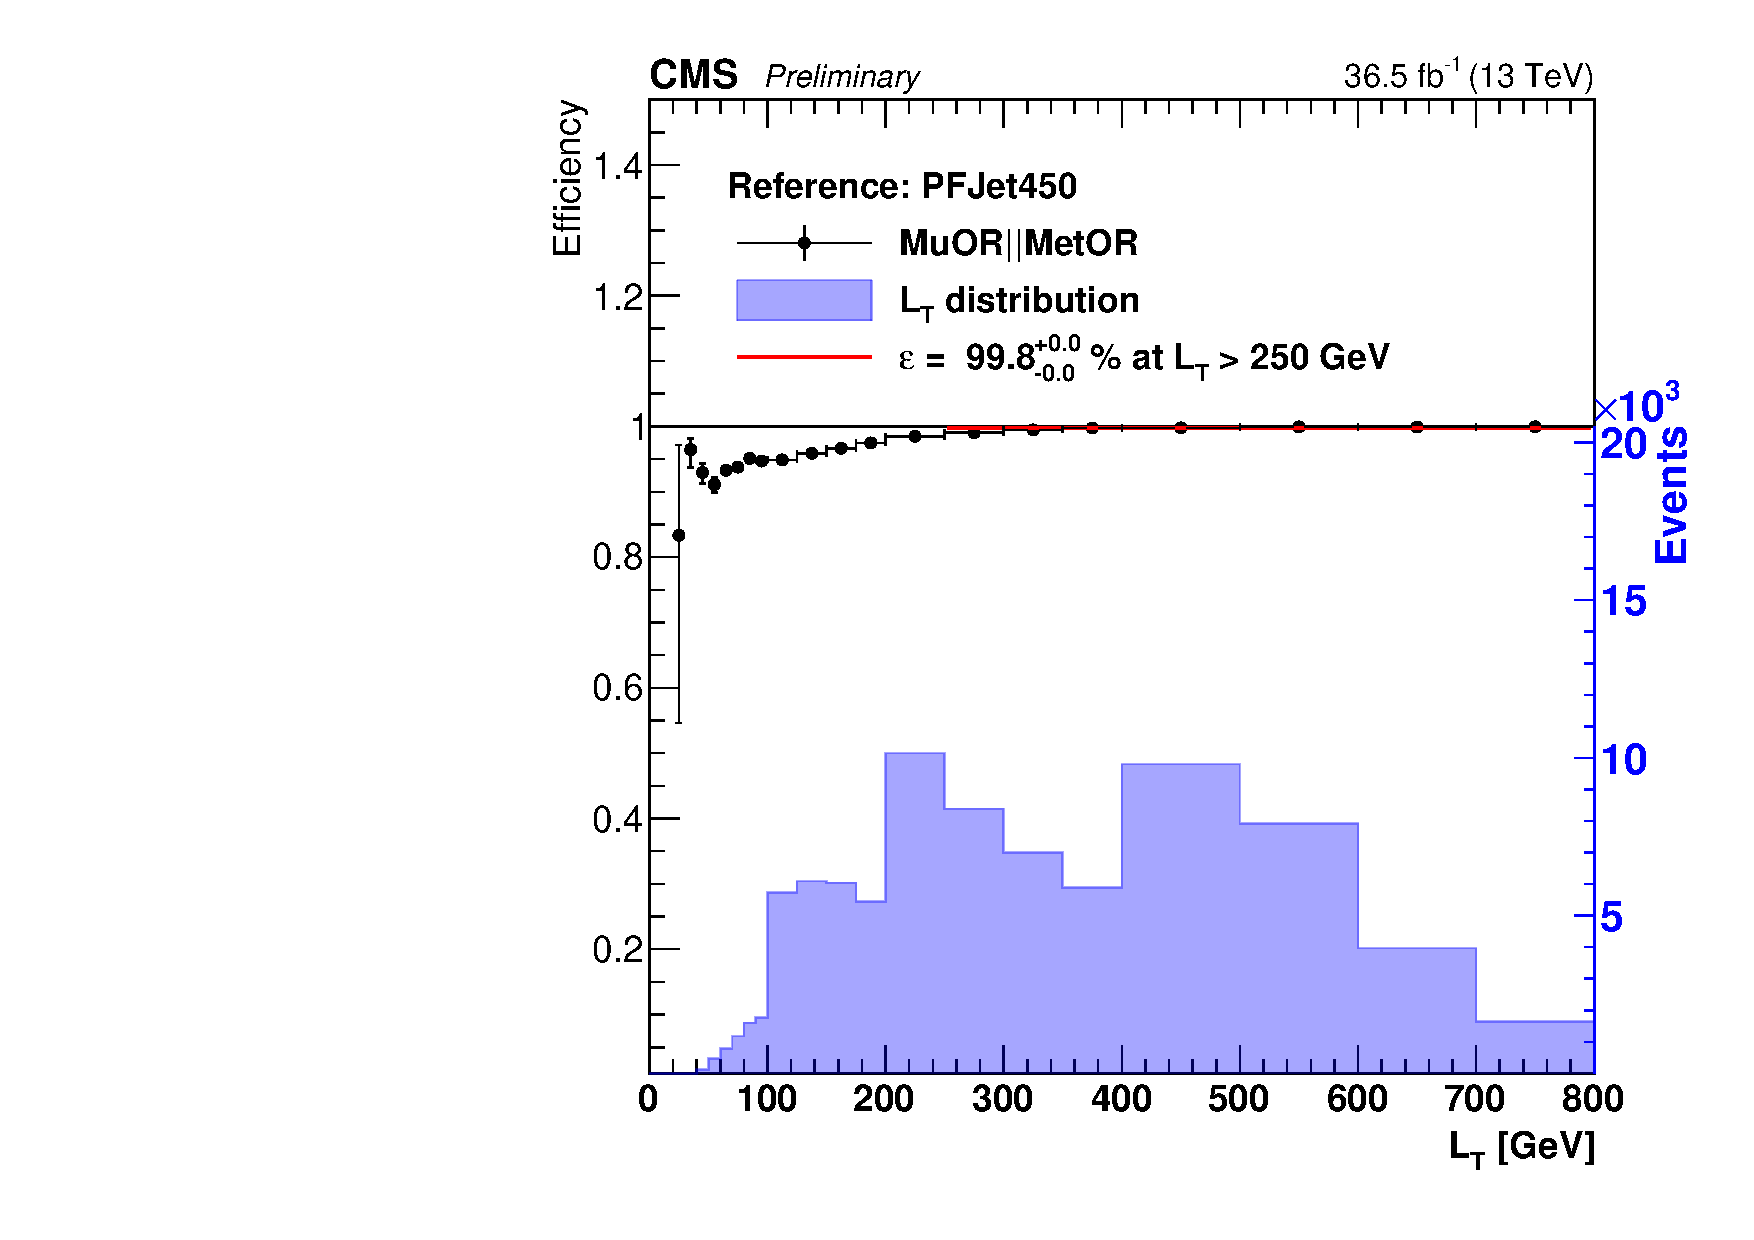
\includegraphics[width=0.4\textwidth]{Plots/trigger/LT_PFJet450_EffFit_test_HLT_MuORORHLT_MetOR.pdf}
  \end{center}
  \caption{Measurement of the trigger efficiency as a function of \LT for the
    electron trigger selection (Ele50PFJet165 / IsoEle27 / Ele105 / Ele115 /
    Ele15HT400 / Ele15HT350 / METMHTTriggers) on the left and the muon trigger
    selection (Mu50 / IsoMu24 / Mu15HT400 / Mu15HT350 / METMHTTriggers) on the
    right \cite{trigger}.
    %The number of events passing the trigger selection is given as shaded
    %histogram
  \label{fig:trig_eff_LT}}
  \end{figure*}
\begin{figure*}[!hbt]
  \begin{center}
    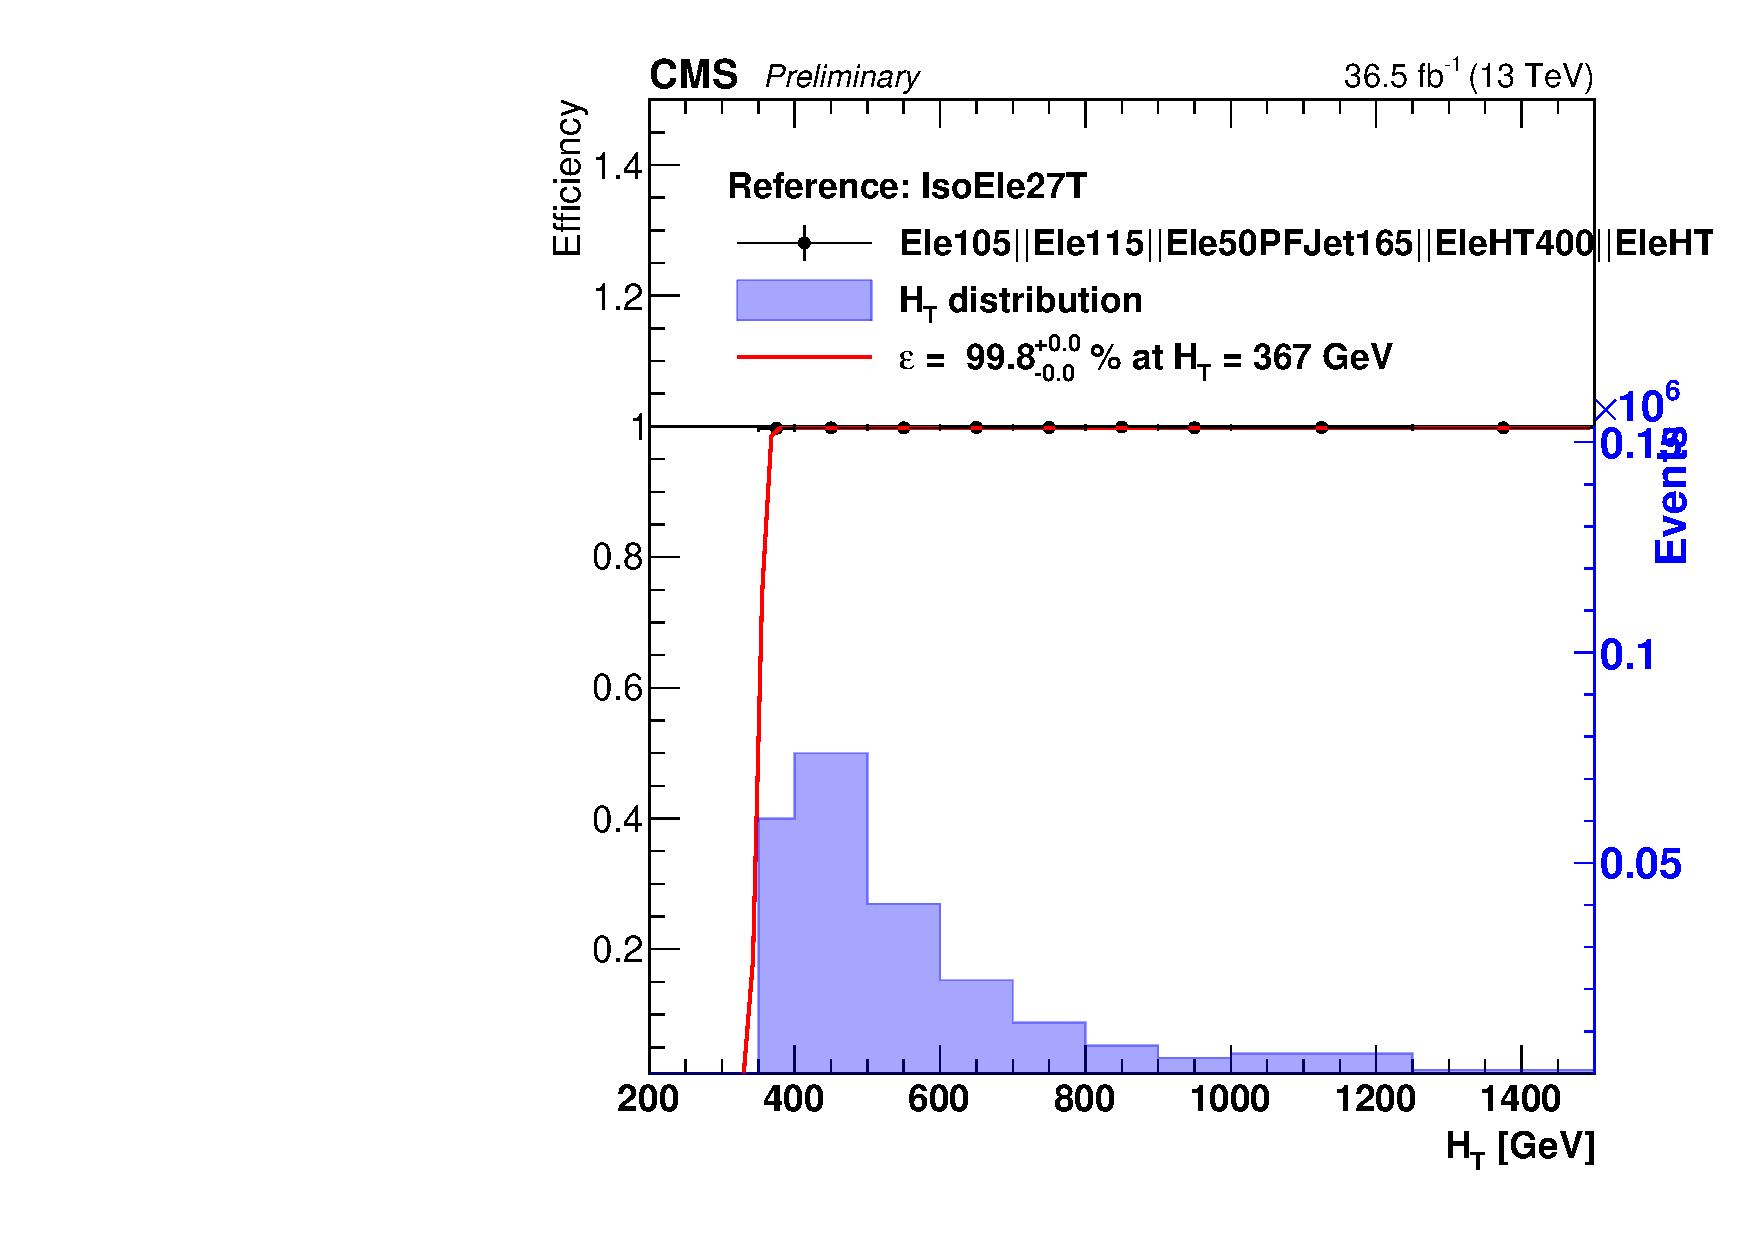
\includegraphics[width=0.4\textwidth]{Plots/trigger/HT_IsoEle27T_EffFit_test_HLT_Ele105ORHLT_Ele115ORHLT_Ele50PFJet165ORHLT_EleHT400ORHLT_EleHT350ORHLT_MetOR.pdf}
    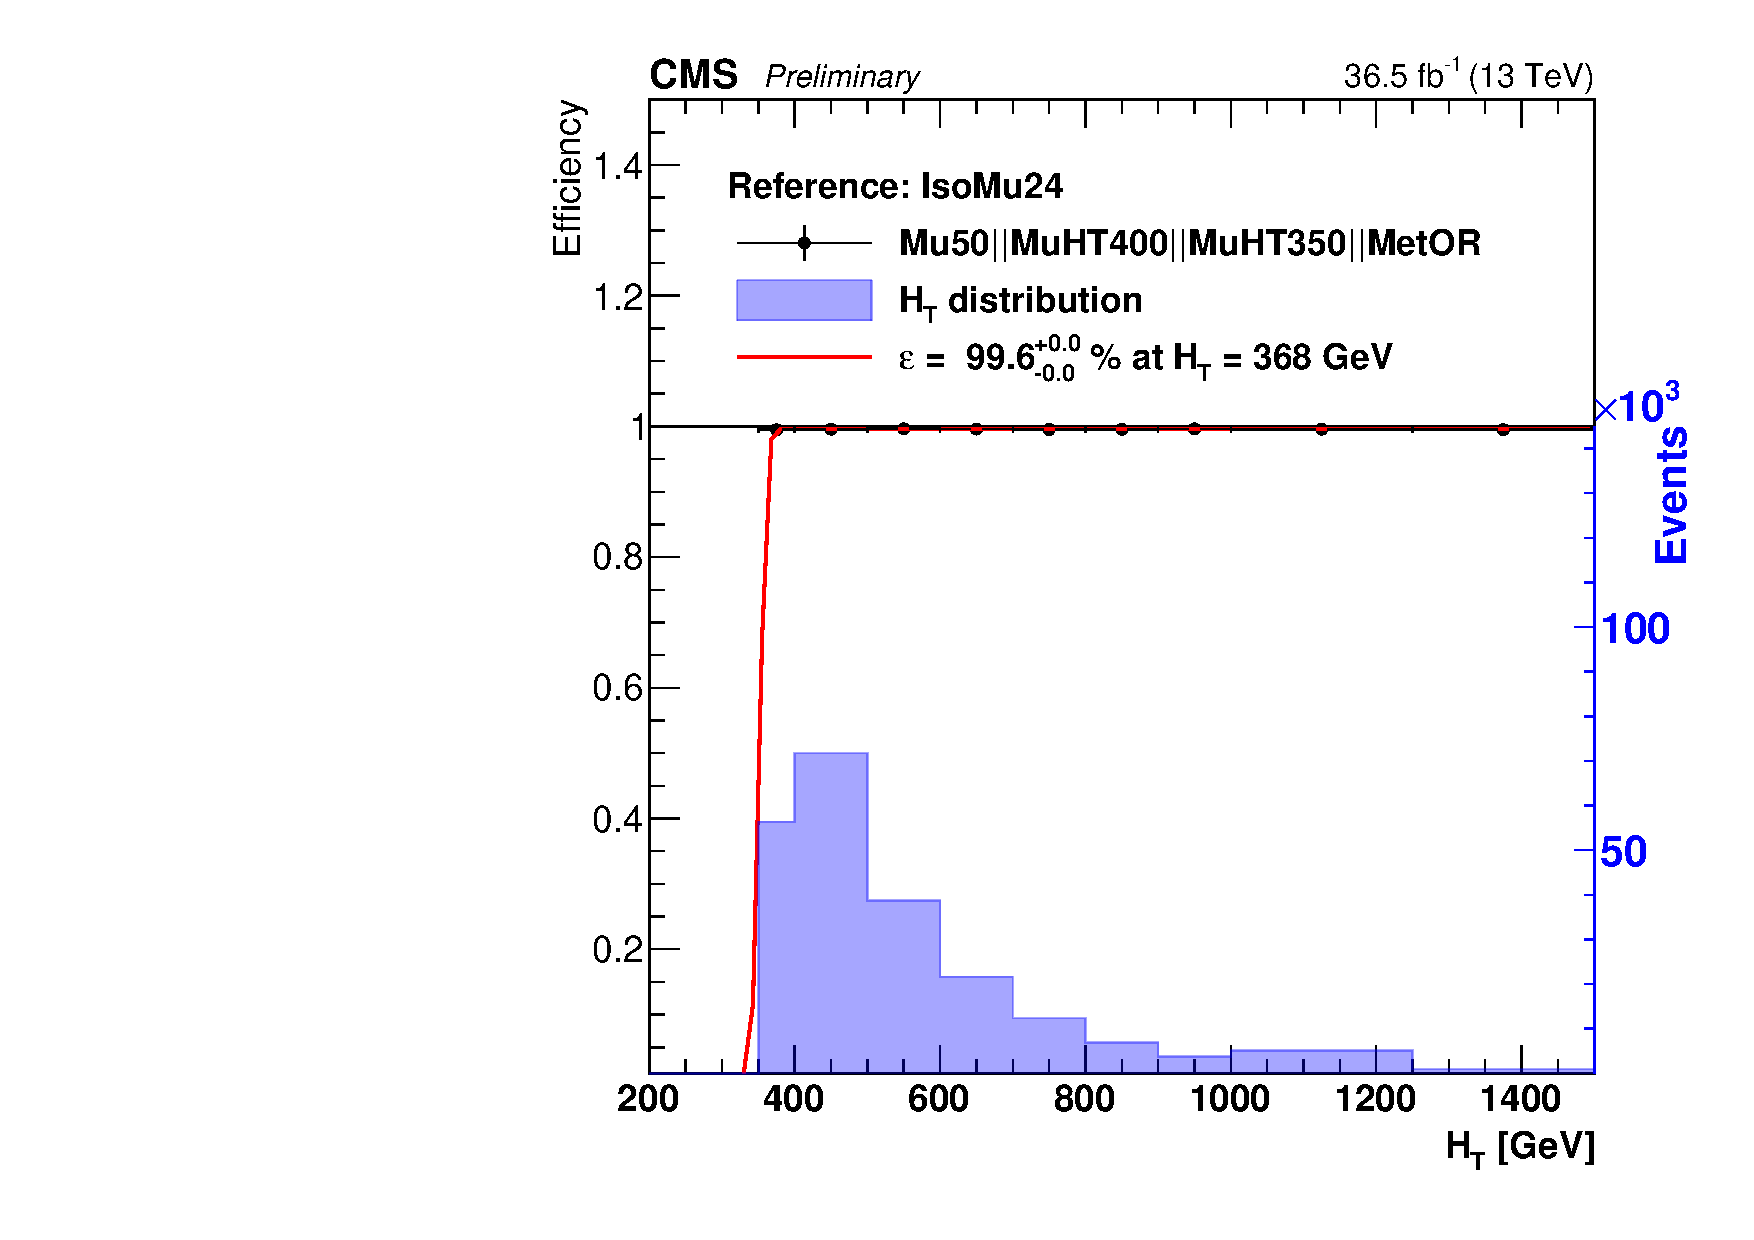
\includegraphics[width=0.4\textwidth]{Plots/trigger/HT_IsoMu24_EffFit_test_HLT_Mu50ORHLT_MuHT400ORHLT_MuHT350ORHLT_MetOR.pdf}
  \end{center}
  \caption{Measurement of the trigger efficiency as a function of \HT for the
    electron trigger selection (Ele50PFJet165 / IsoEle27 / Ele105 / Ele115 /
    Ele15HT400 / Ele15HT350 / METMHTTriggers) on the left and the muon trigger
    selection (Mu50 / IsoMu24 / Mu15HT400 / Mu15HT350 / METMHTTriggers) on the
    right \cite{trigger}.
    %The number of events passing the trigger selection is given as shaded
    %histogram
  \label{fig:trig_eff_HT}}
  \end{figure*}
  \begin{figure*}[!hbt]
    \begin{center}
    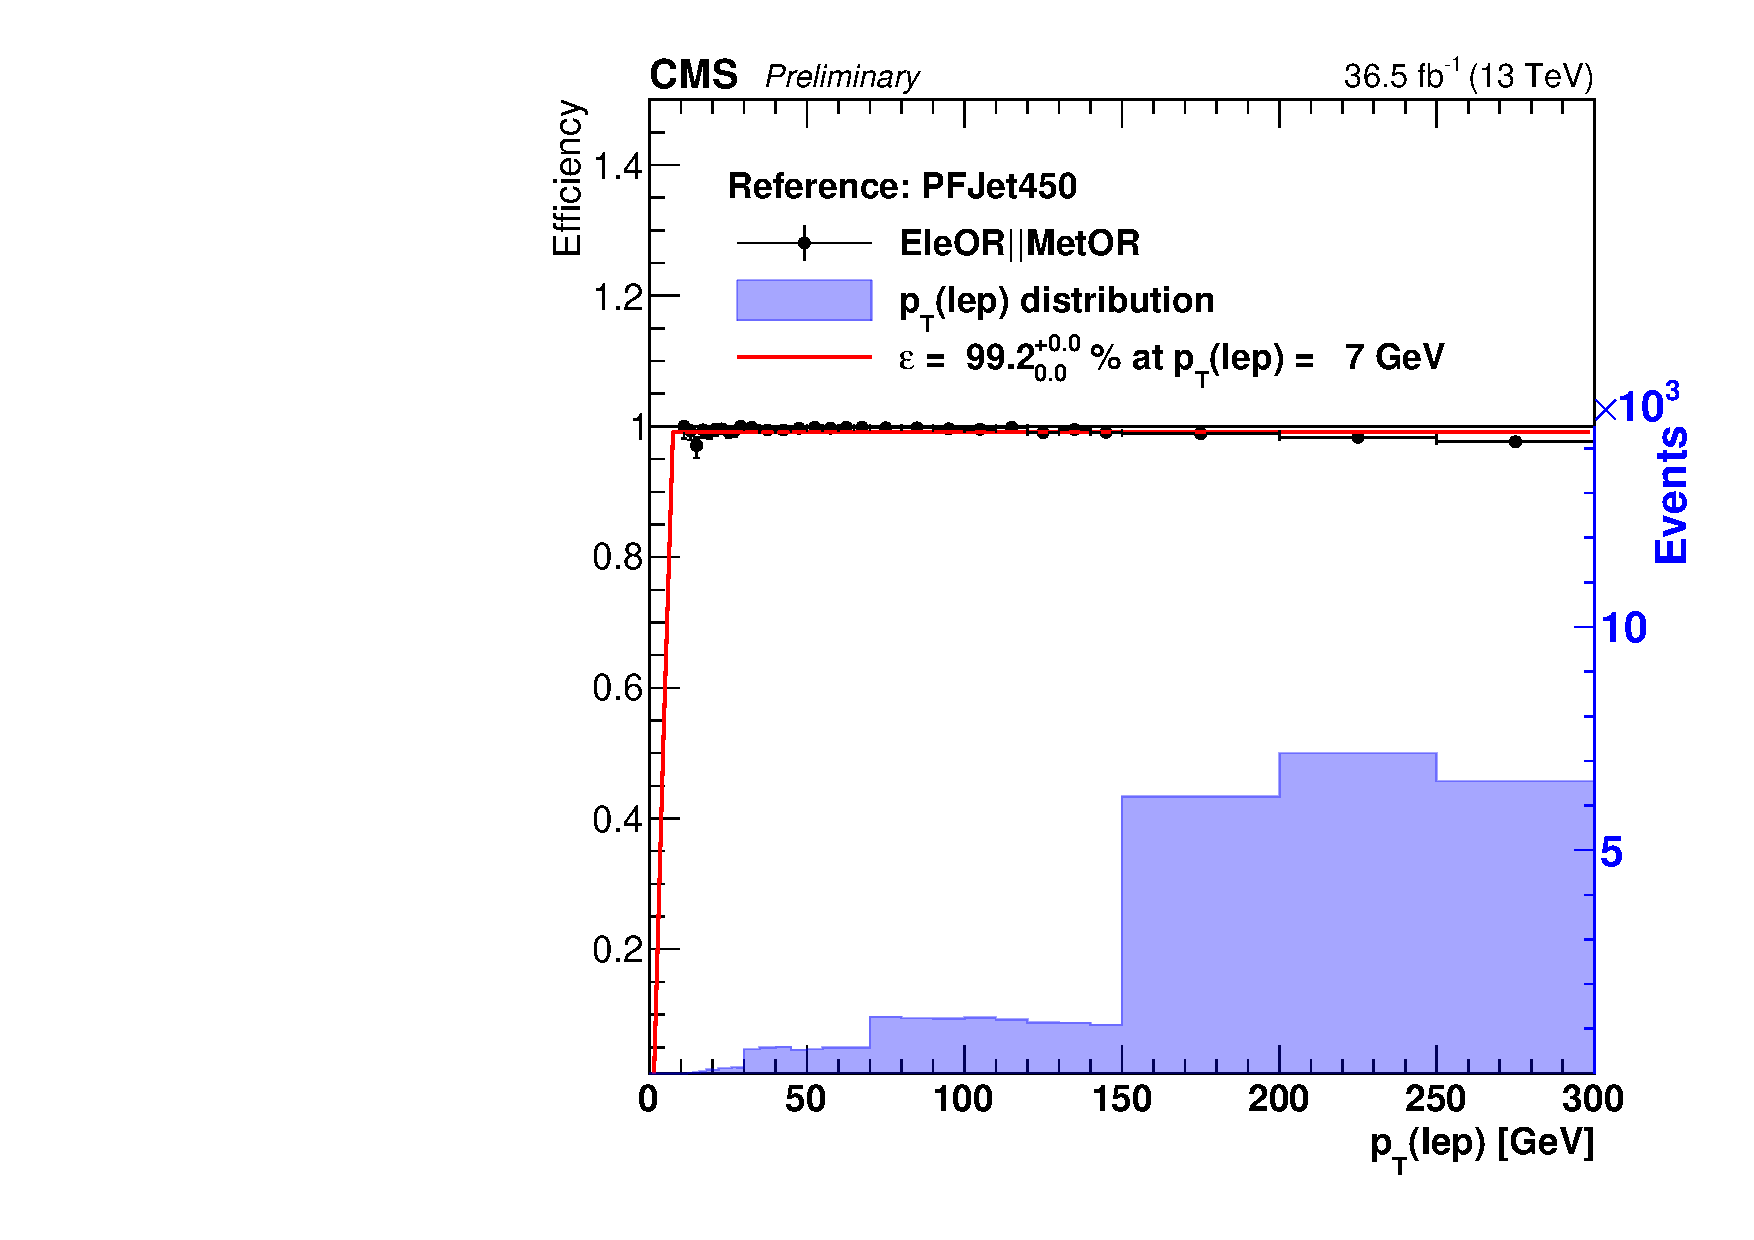
\includegraphics[width=0.4\textwidth]{Plots/trigger/LepPt_PFJet450_EffFit_test_HLT_EleORORHLT_MetOR.pdf}
    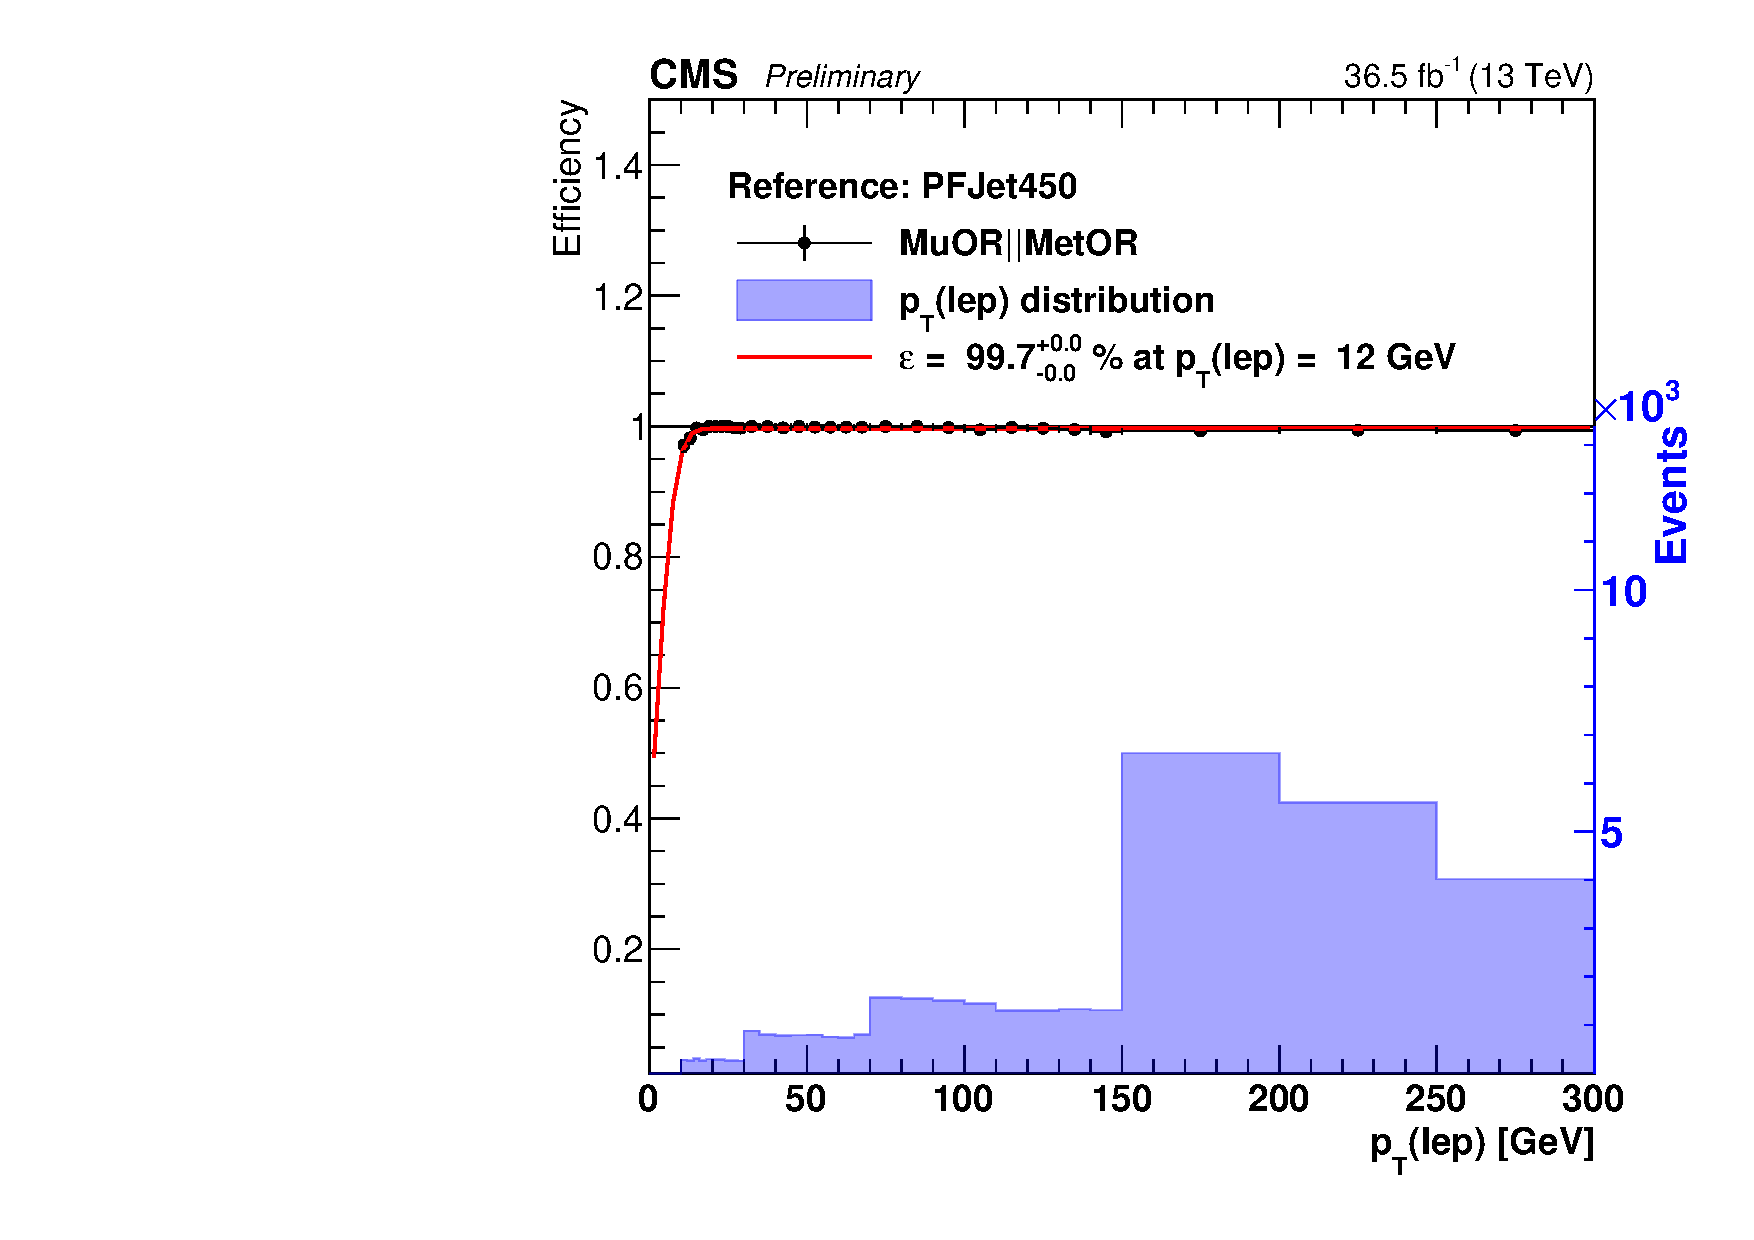
\includegraphics[width=0.4\textwidth]{Plots/trigger/LepPt_PFJet450_EffFit_test_HLT_MuORORHLT_MetOR.pdf}
  \end{center}
  \caption{Measurement of the trigger efficiency as a function of lepton $p_T$ for the
    electron trigger selection (Ele50PFJet165 / IsoEle27 / Ele105 / Ele115 /
    Ele15HT400 / Ele15HT350 / METMHTTriggers) is shown on the left and the muon trigger
    selection (Mu50 / IsoMu24 / Mu15HT400 / Mu15HT350 / METMHTTriggers) is shown on the
    right. The lepton $p_T$ trigger efficiency is measured after an $\LT>250$\,GeV cut which is the analysis baseline selection \cite{trigger}.
    %The number of events passing the trigger selection is given as shaded
    %histogram
  \label{fig:trig_eff_leptonPt}}
\end{figure*}
\section{Event cleaning: Filters}
\label{sec:filters}
The event reconstruction can fail due to the noisy detector cells and other kinds of detector problems. These can result in incorrectly reconstructed physics objects such as: muons, jets and hence MET. In CMS, the physics object groups related to the problem release event filters or cures for the falsely reconstructed objects. \\
\textbf{Primary vertex filter:}\\
A good primary vertex is required which is introduced in section \ref{sec:PV}.\\
\textbf{Beam halo filter:}\\
The collisions of the beam with residual gas inside LHC cause showers of secondary particles. Additionally to these scattering effects, charged particles are deflected by the magnetic field of the beam optics. These particles are called beam halo particles and one of the main sources of the beam background of the LHC. In CMS, the beam halo algorithm considers the particles produced outside the CMS cavern and to detect events with beam halo it uses the timing information and hit topology in CSC, ECAL and HCAL subsystems. 
\textbf{HB-HE noise filter:}\\
This noise is originated from the Hybrid PhotoDiodes and Readout Boxes of the HCAL. The timing, pulse shape as well as the other readout errors are used to detect the noise. \\
\textbf{ECAL dead cell trigger primitive filter:}\\
The existence of noisy crystals in ECAL can lead to fake MET. The events, in which the noisy cells deposit high energy, are filtered.\\
\textbf{Bad PF muon filter:}\\
This filter fires when there is a PF muon with too low quality and has large $\pt$. The quality of the muon is determined according to its tracking uncertainty, segment compatibility and other detector related features. This bad muon is required to have $\pt > 100$ GeV. Unlike the other filters explained above this filter is applied to background simulation samples as recommended. \\
\textbf{Bad charged hadron filter:}\\
The events, where there is a muon but it fails to be a PF muon and it still contributes to PF MET calculation as a charged hadron candidate, are filtered. Here, as in the previous case, this muon is required to have $\pt > 100$ GeV. Moreover, it is required that the muon and the charged hadron traces are almost overlapping ($\Delta R(\mu, charged\, hadron)<$ 0.00001). In addition to this, their $\pt$s are needed to be very close to each other. Similarly to the bad PF muon filter, this is applied to background MC samples as well as the data events. \\
\textbf{Duplicate muon filters:}\\
In the Re-reco data it is observed that there is an increase in events in the MET tail of Z$\rightarrow\mu\mu$ data. It is understood by the muon POG that there are dublicate muons in the events due to reconstruction failures. 
Additionally, two filters are recommended by the SUSY group:  
One is to remove events with the ratio of PF MET to calorimeter MET is more than 5.  The second is to remove events containing bad jets which have $\pt > 200$ GeV, muon energy fraction $>0.5$ and $\Delta\phi(met,jet)>\pi-4$.\\
\textbf{Filter on fastsim:}\\
This filter is to clean up bad jets from the fastsim events. To remember, in this work, fastsim is used for the signal MC production. The event is removed if there is a jet satisfying the following conditions:  $\pt > 20$ GeV, $|\eta|<2.5$, unmatched to a generated jet ($\Delta R(jet,gen\,jet)>0.3$), and charged hadron fraction $<$ 0.1.
\\
\\
The efficiency of all these filters after the analysis baseline selection is approximately 98\%.

\section{Control plots}
The distributions of main kinematic variables, also called control plots, are shown in this section. In all the control plots, the colored lines represent the signal models and the color filled stacked histograms display the background processes. Additionally, the black dotted distribution exhibits the observed data points requiring the triggers introduced in section \ref{sec:triggers}. In all the control plots, the events are cleaned by the filters discussed in section \ref{sec:filters}. The signal and background events are scaled by the luminosity factor and additional weights introduced in section \ref{sec:SF}. In the Figure \ref{fig:baselineplots} top left plot shows the n-btag distribution after the baseline selection (see section \ref{sec:BL}). The distribution of simulated signal events peaks at zero as expected. Clearly, one can see from this distribution that choosing events with zero b-tagged jets suppresses the $\ttbar$ background significantly. The other distributions, displaying main kinematic variables, exhibit reasonable MC-data agreement although it is not necessarily expected. The plot shows the number of jet distribution (top/right), $\HT$ (bottom/left) and $\LT$ (bottom/right) are shown. \\
The multiplicities of jets and b-tagged jets display no difference between the signal scenarios, since the mass splitting has no effect on the decay topology. 
The two selected signal benchmark models show differences in the distributions of $\HT$ and $\LT$, this is due to the gluino-neutralino mass splitting. In the non-compressed T5qqqqWW (1900,100) model, the quarks coming from the gluino decay have a large boost, resulting in high leptonic and hadronic energy scales. For the compressed region with T5qqqqWW (1500,1000) no such effect is observed, and the shape of the distributions look similar to the SM processes. \\
Additional control plots are shown in Appendix \ref{sec:CRplots}. 
 \begin{figure*}[!hbt]
    \begin{center}
 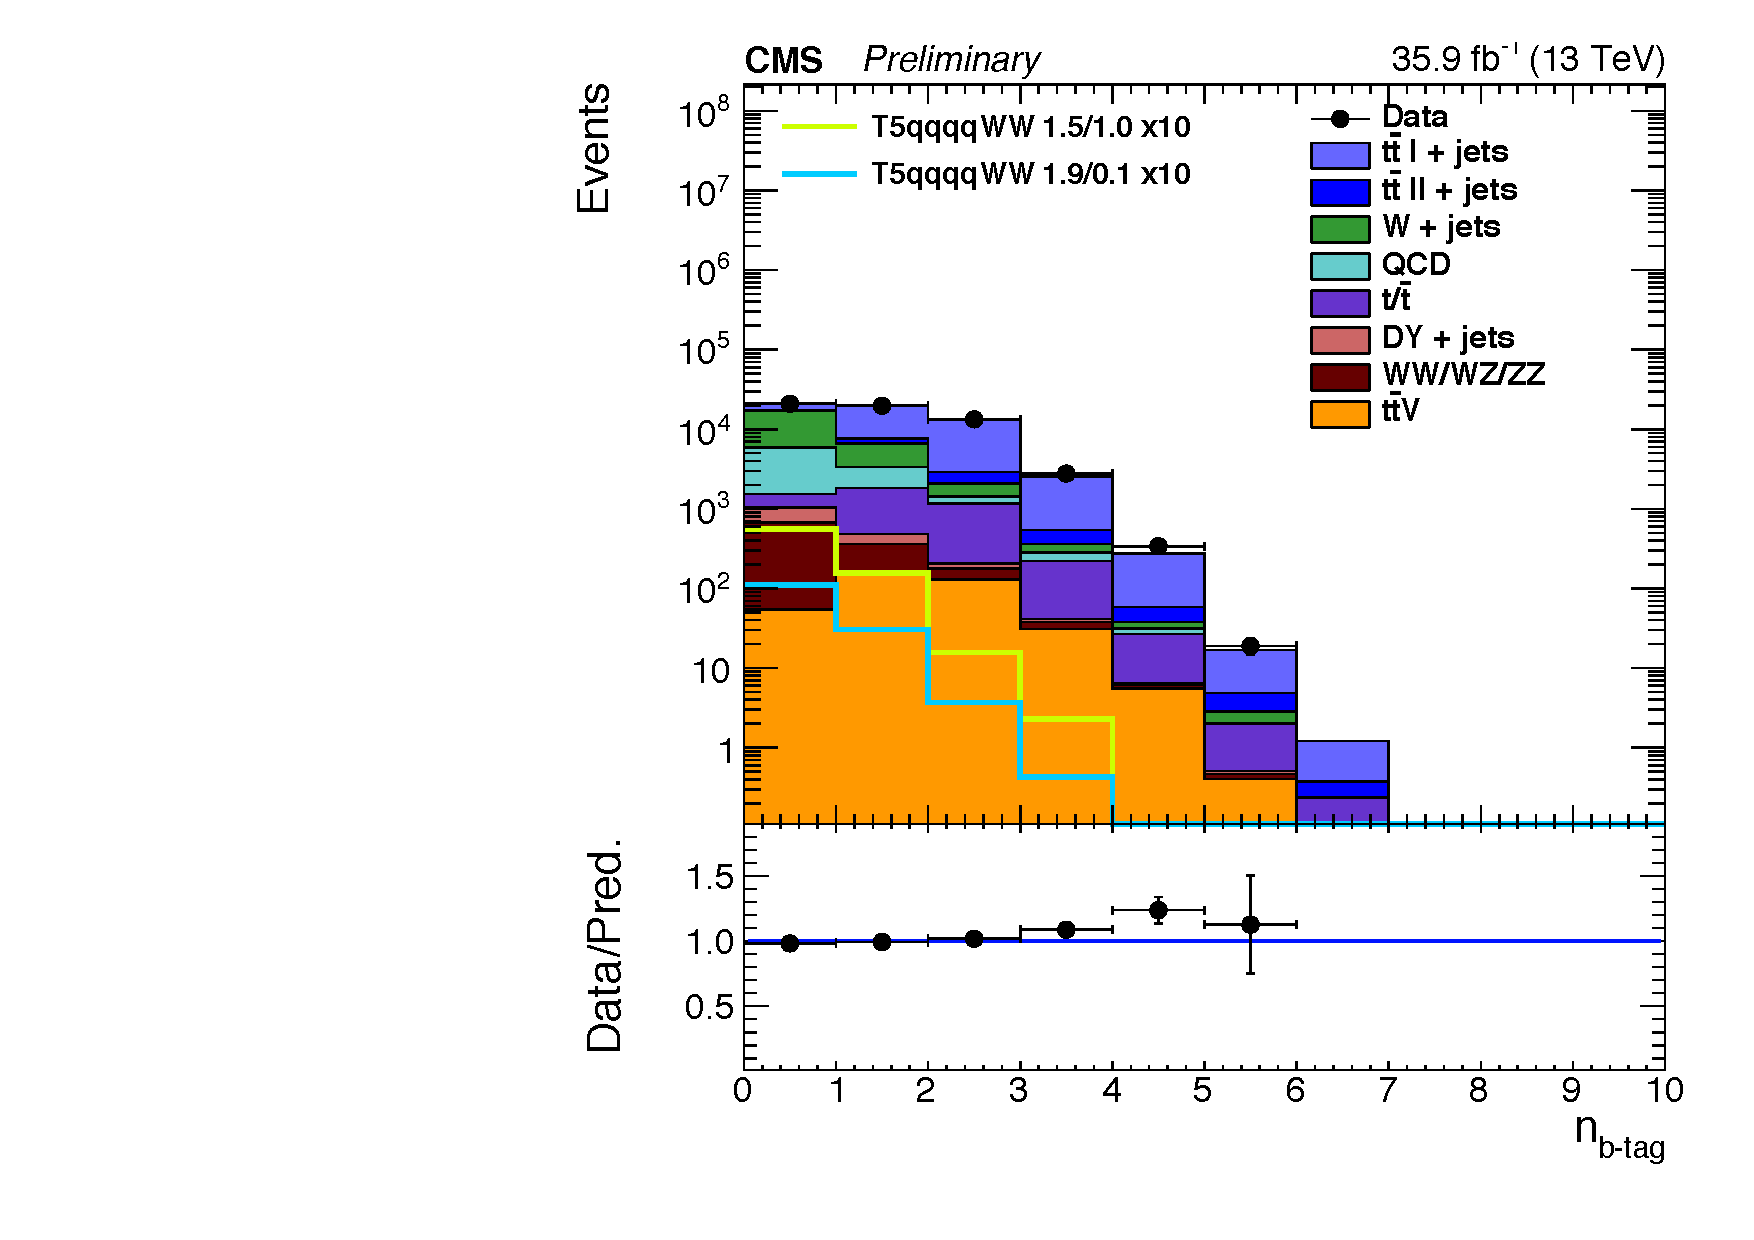
\includegraphics[width=0.45 \textwidth]{Plots/analysis/control_Plots/nBjet0b}
 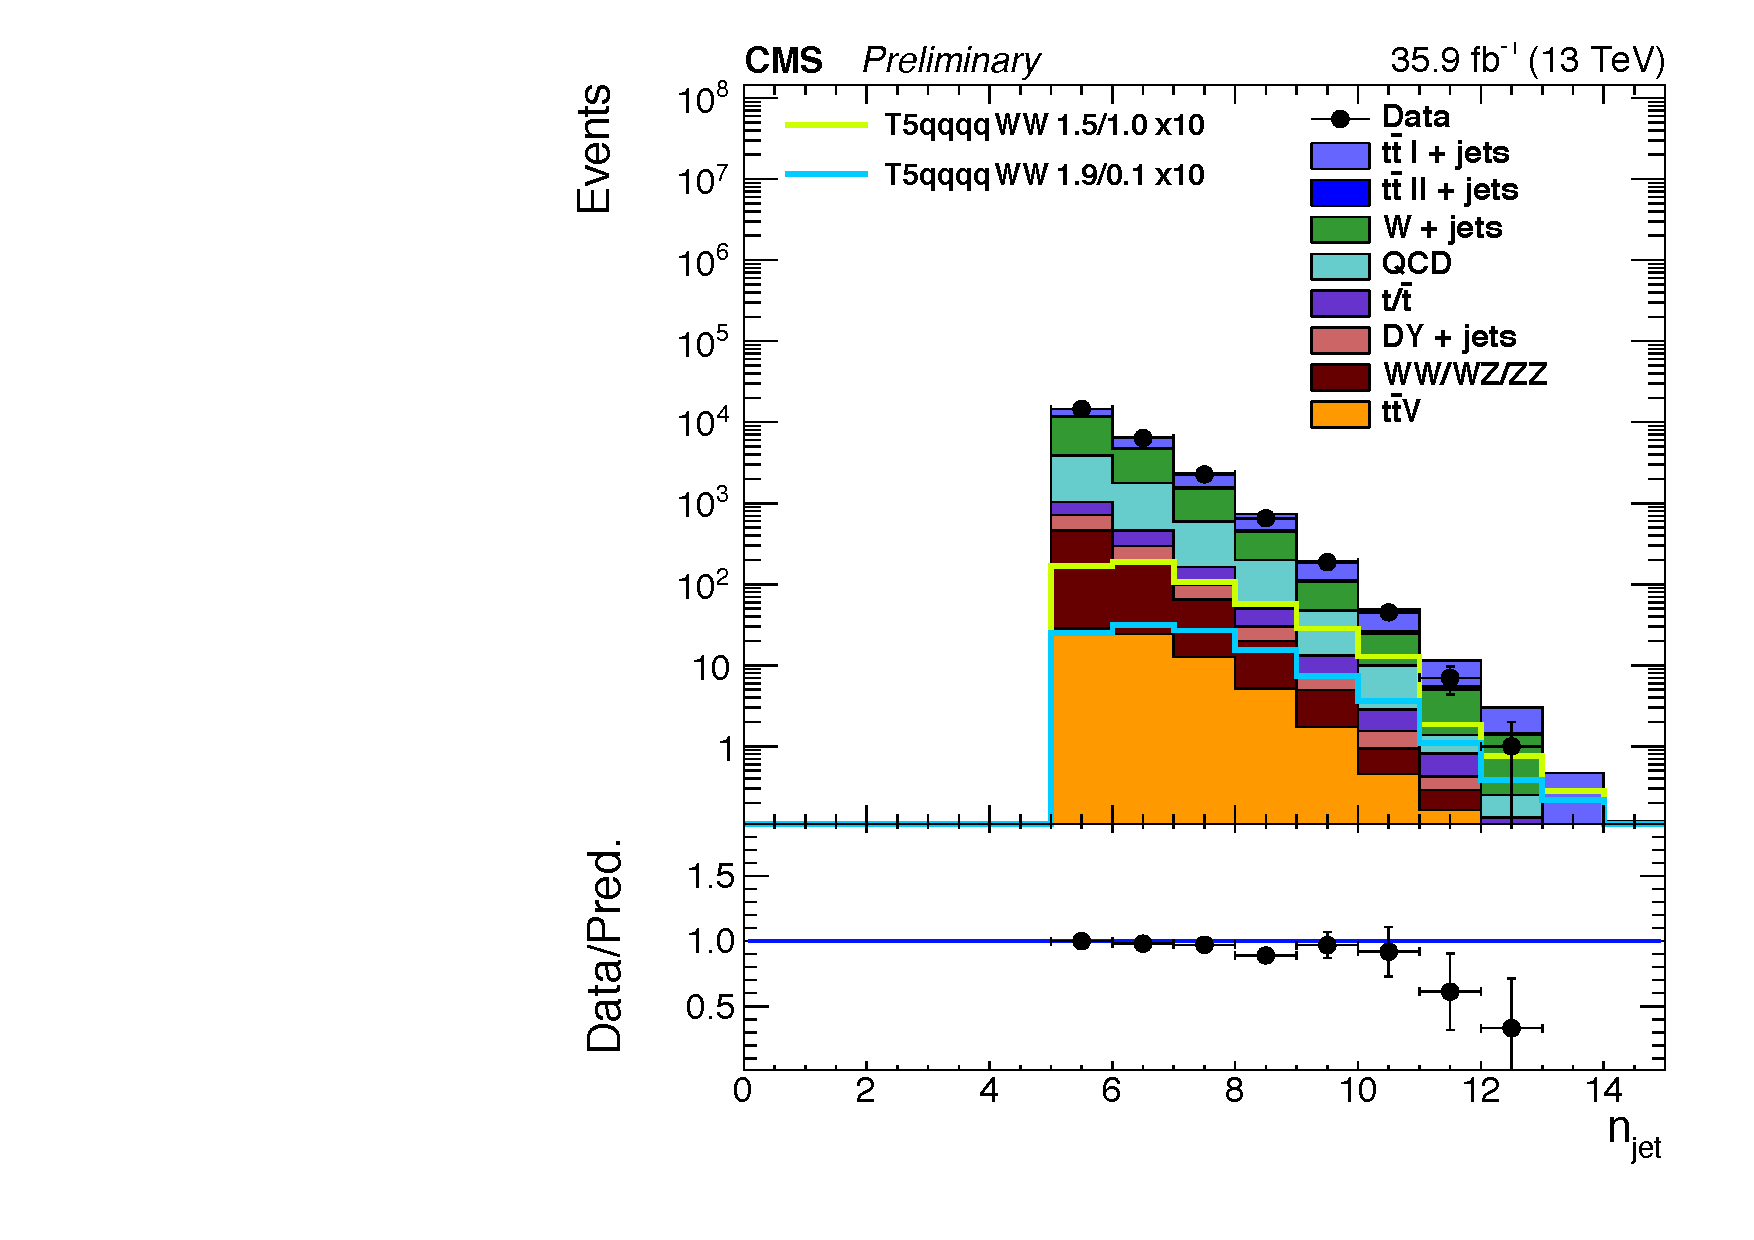
\includegraphics[width=0.45 \textwidth]{Plots/analysis/control_Plots/plots_zerob_st250_ht500_njet5_nbtagEq0_nJet30Preliminary}\\
 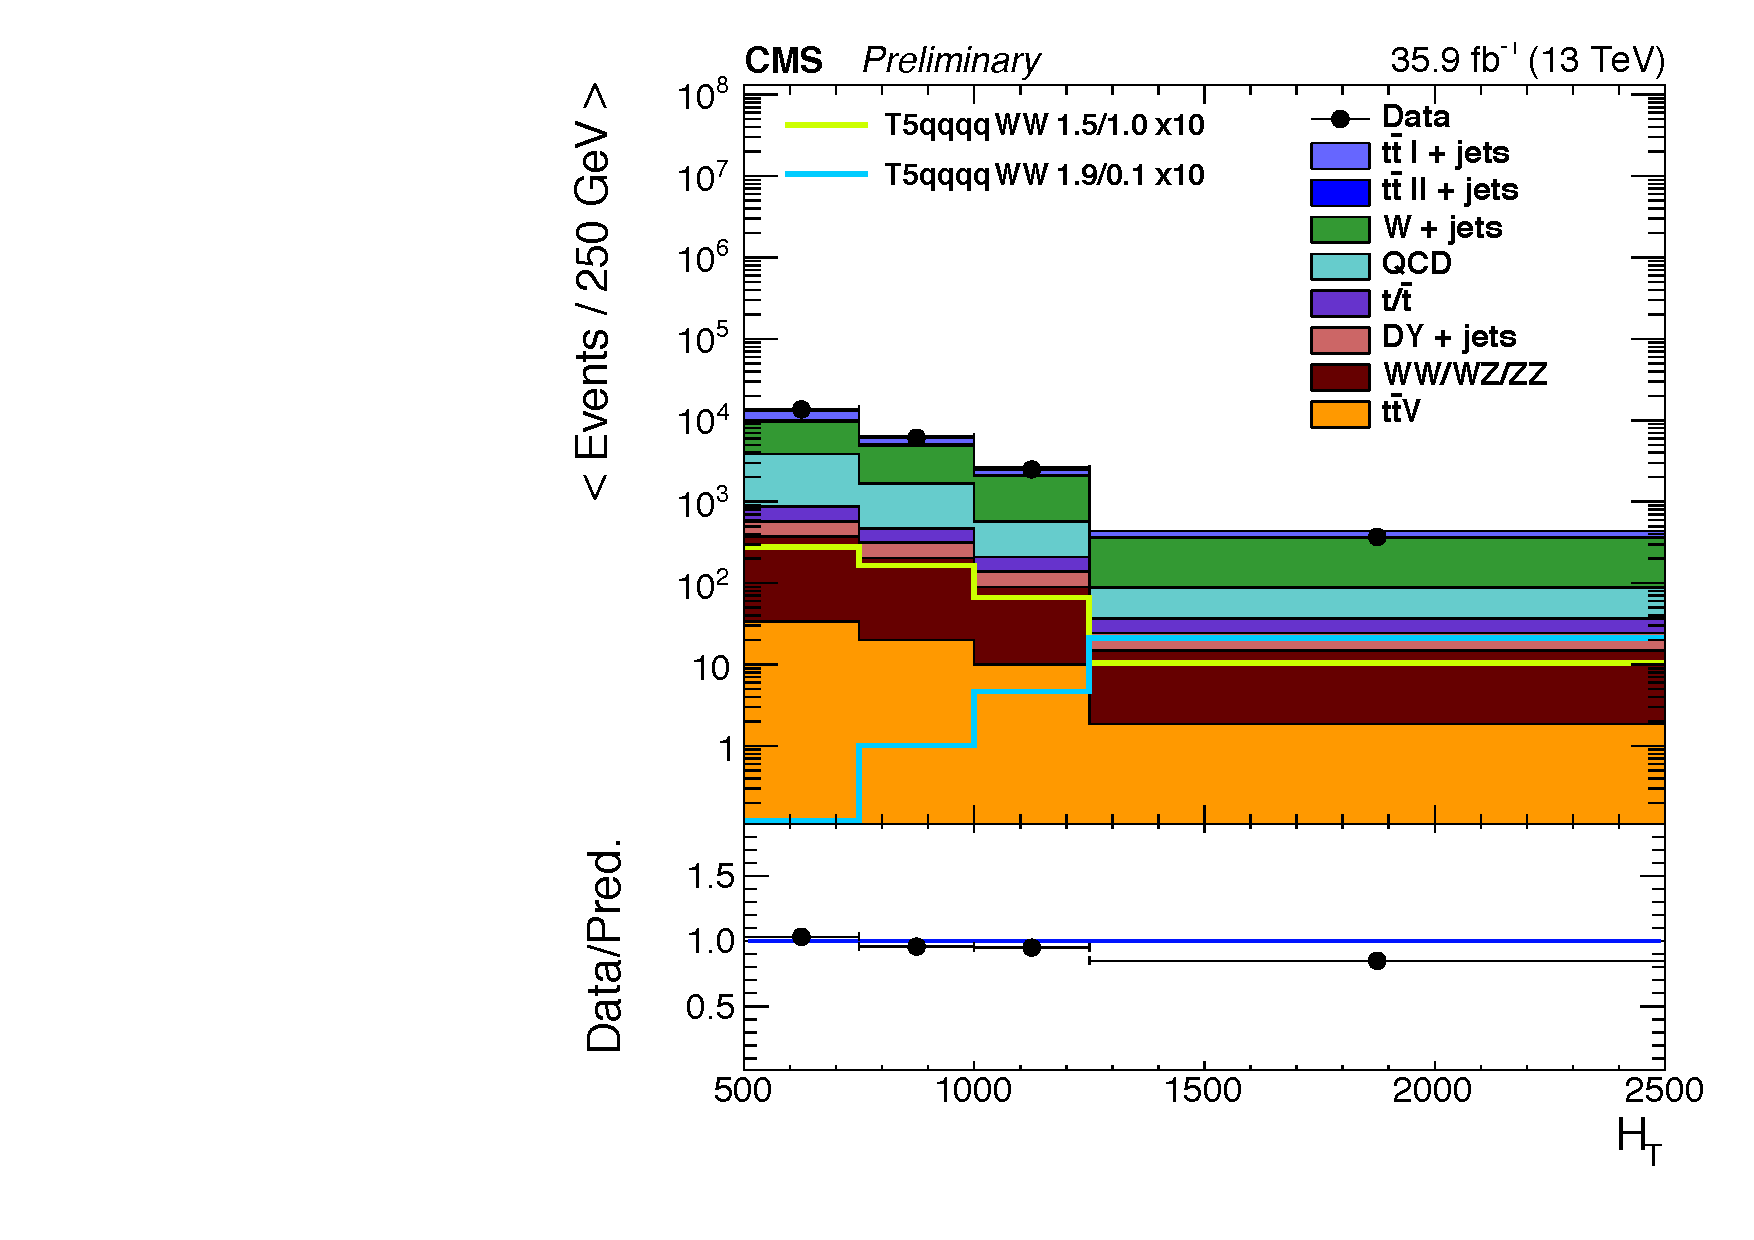
\includegraphics[width=0.45 \textwidth]{Plots/analysis/control_Plots/plots_zerob_st250_ht500_njet5_nbtagEq0_htJet30jPreliminary}
 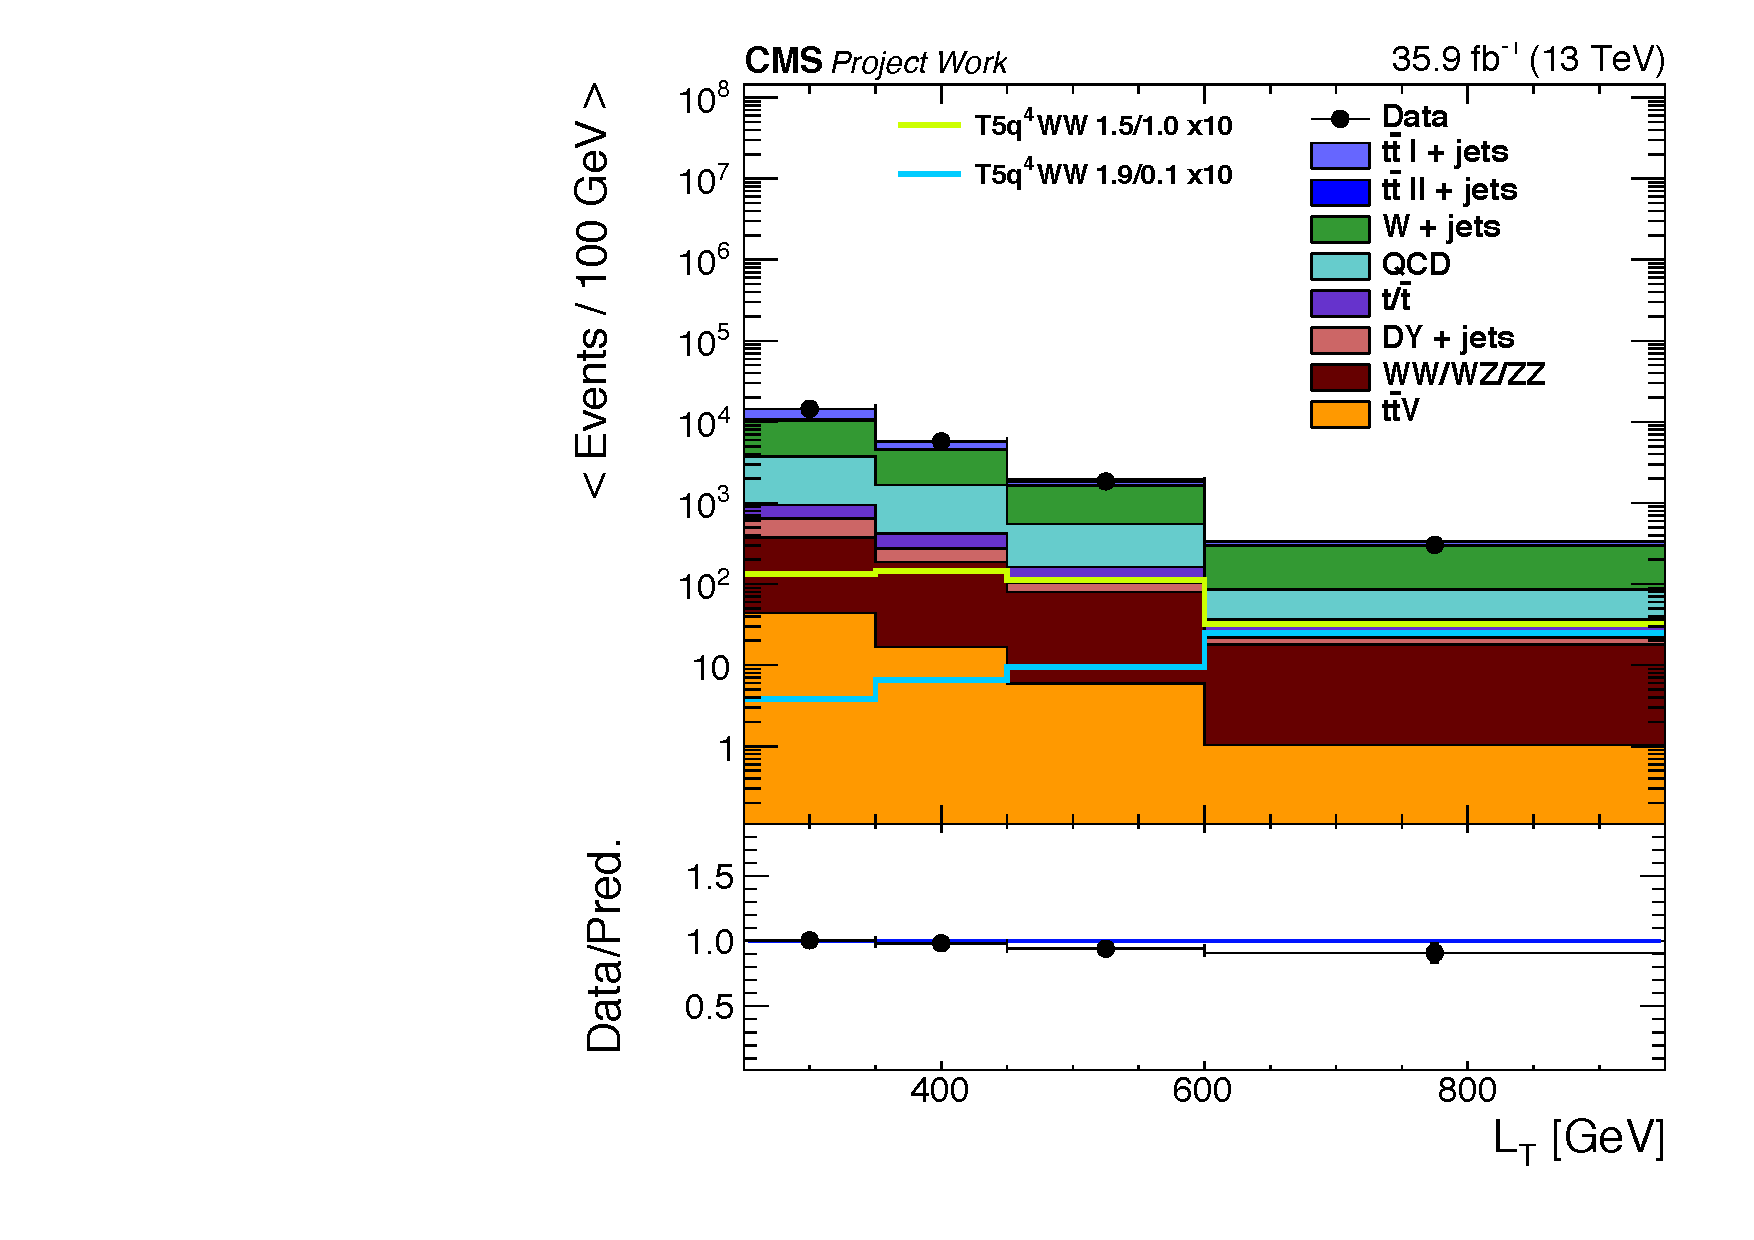
\includegraphics[width=0.45 \textwidth]{Plots/analysis/control_Plots/LT_colors}
 %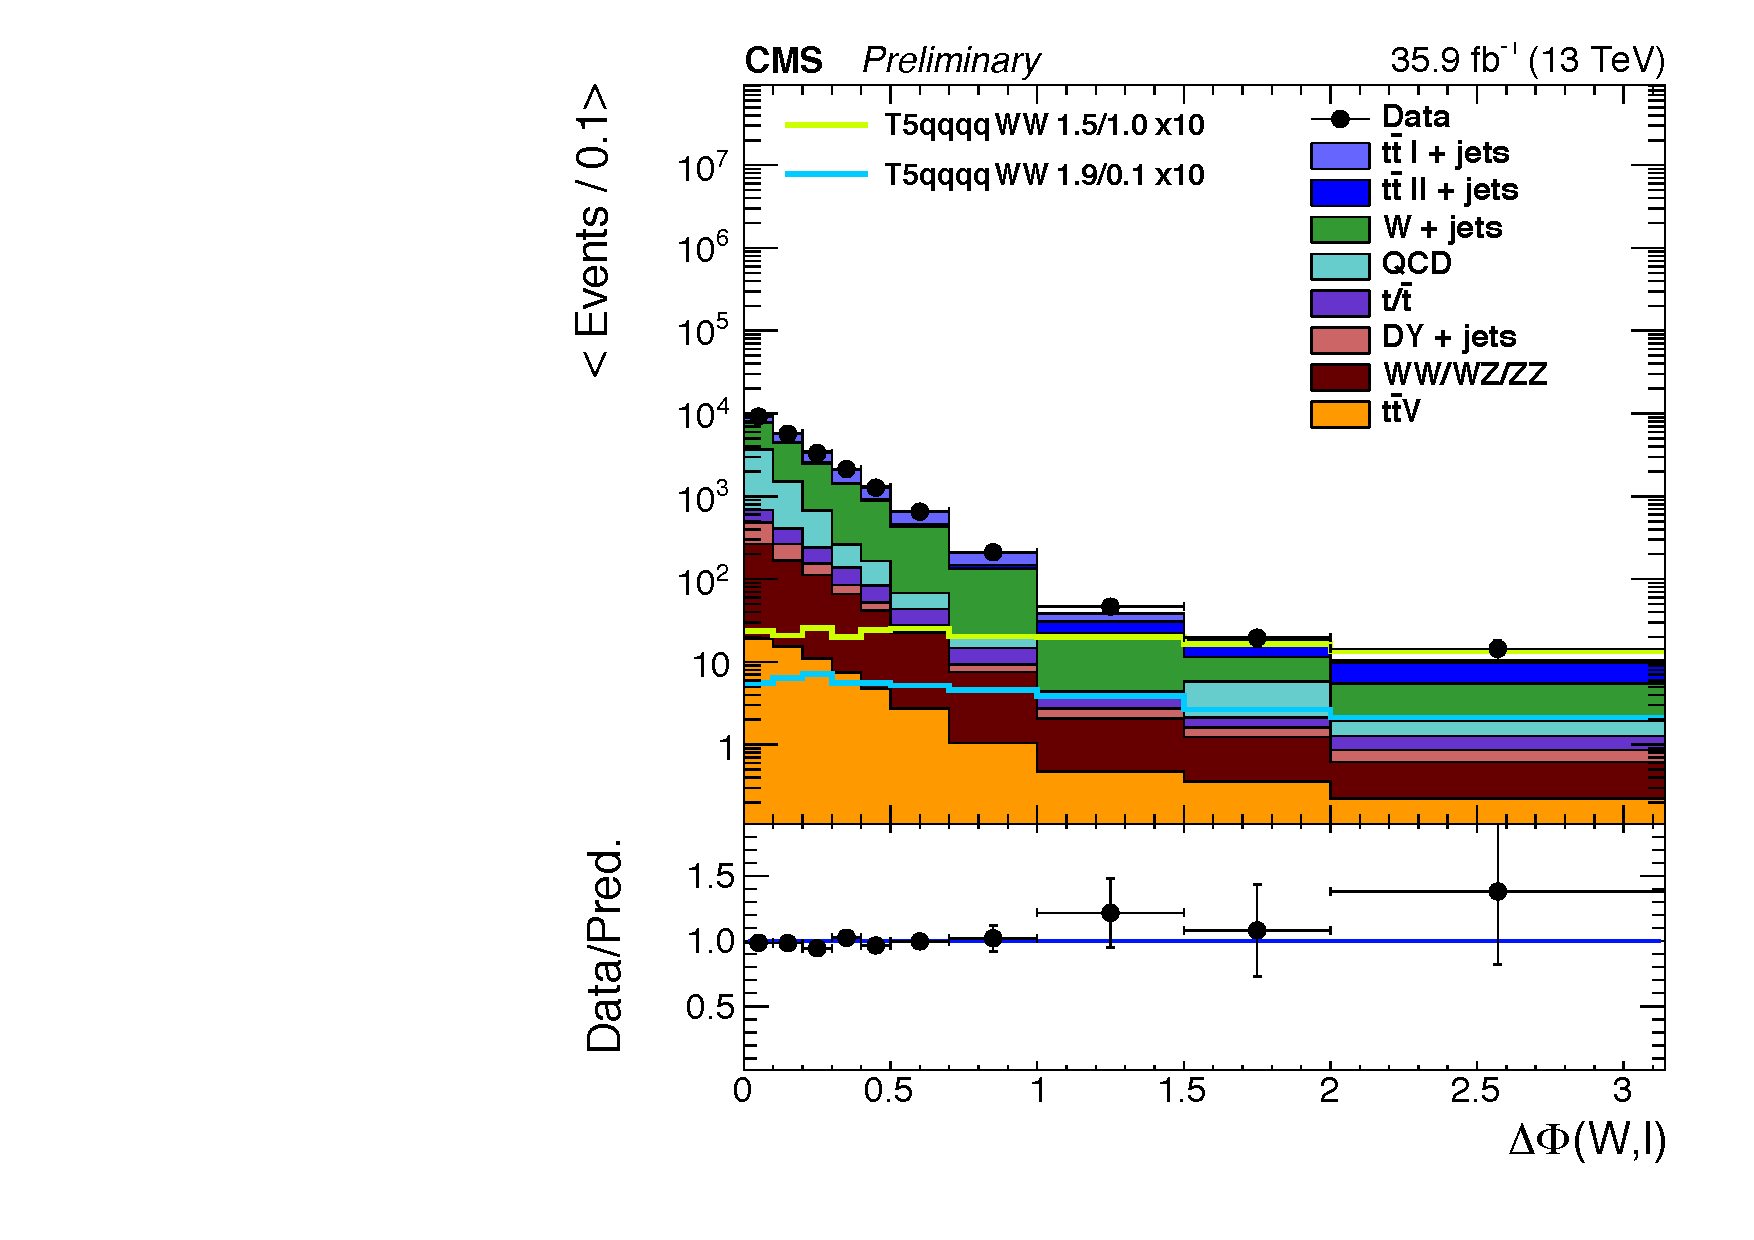
\includegraphics[width=0.45 \textwidth]{Plots/analysis/control_Plots/plots_zerob_st250_ht500_njet5_nbtagEq0_deltaPhi_WlPreliminary}
  \caption{ \label{fig:baselineplots} The top left distribution shows the number of b-tagged jets, after the baseline selection, requiring at least five jets, minimum $\HT$ of 500 GeV, a minimum $\LT$ of 250 GeV and exactly one lepton with $\pt >$25 GeV. The rest of the distributions are plotted after the same baseline selection additionally requiring no b-tagged jets. In the top row the number of jets (right) while in the bottom row $\HT$ (left) and $\LT$ (right) distributions are shown. The simulated background events are stacked on top of each other, and several signal points are overlaid for illustration without being stacked. The model T5qqqqWW (1.5,1.0) (T5qqqqWW (1.9,0.1)) corresponds to a gluino mass of 1.5 TeV (1.9 TeV) and neutralino mass of 1.1 TeV (0.1 TeV), respectively. The intermediate chargino mass is fixed at 1.25 TeV (1.0 TeV). The two benchmark signal models are scaled up by a factor of 10.
  }
   \end{center}
\end{figure*}
\chapter{Design of Search Regions}
Explain MB , SB...  
\newpage
\section{Signal Regions}
\subsection{Background and Signal composition in MB SR}
\newpage
\section{Control Regions}
\subsection{Background composition in MB CR and SB SR/CR}
\newpage
\newpage
\subsection{Signal contamination in MB CR and SB SR/CR}
Tell that It is negligible
\newpage
